\chapter{Results}

\section{Deuteron photodisintegraion}

    \subsection{Cross section}
    \label{cross_results}

    In this section I will show the results of my calculation starting from the
    deuteron photodisintegration process. One of the most
    studying observable is obviously the cross section. There is
    a number of papers which present 
    measurement results for both differential and total cross section
    \cite{BOSMAN1979,ARENDS1984,Skopik1974, Moreh1989, Birenbaum1985, Bernabei1986, rachek2007,Ying_Experiment_Deut, DeSanctis_Experiment_Deut} 
    and it seems interesting to compare 
    our predictions with experimental results.

    In Fig.~\ref{TOTAL_CROSS_small} and Fig.~\ref{TOTAL_CROSS} 
    I present predictions for the
    total cross section $\sigma_{tot}~[\mu\text{b}]$ which I obtained
    using the chiral potential at the order N$^4$LO+ and with 
    the cutoff parameter $\Lambda=450$~MeV (my best predictions).
    From Fig.~\ref{TOTAL_CROSS_small}, we see that at low photon energies
    (below 50 MeV) predictions which include 2N contributions
    via the Siegert approach, describe experimental results quite well.
    We can suppose that the difference with experimental data may come from 
    the statistical uncertainty of  the data itself, as my predictions
    are often in between the data from different sources.
    Moreover even at such low energies the 1N current is clearly not enough
    to describe this observable as dashed pink line has much lower values and
    the difference becomes even larger with larger photon's energies.
    At 5~MeV the difference between 1N predictions
    and 1N + Siegert is 297.54~$\mu$b (10.8\%), increasing energy to 10 MeV
    it is 304.28~$\mu$b (20.4\%) and at 20~MeV it is 229.50~$\mu$b (39.2\%).
    Even with energy increasing from 5~MeV to 20~MeV -
    the difference between predictions has changed from 10.8\% to 39.2\% and
    from \fig{TOTAL_CROSS_small} we see that the gap  continues increasing even more with larger energies.

    Here and later the relative difference between set of predictions ($x_1$, $x_2$, ..., $x_N$) is calculated
    using the formula:

    \begin{equation}
        \Delta = \frac{\max(x) - \min(x)}{\frac{1}{N}\sum_{i=1}^N x_i} \cdot 100\%
    \end{equation}


    Having look at the higher energies (above 50~MeV, Fig.~\ref{TOTAL_CROSS})
    we can notice that the discrepancy with experimental data is not only 
    quantitative, but also qualitative.  There is a peak around 300~MeV
    in the experimental data from \cite{Bernabei1986} which is not
    reflected in my predictions. The reason of such discrepancy 
    is most likely coming from the relativistic effects
    which I do not take into account. At higher energies their contribution
    becomes larger and here we observe a clear justification of such a lack.
    It is also confirmed by the calculations in \cite{ArenhovelPhotodisint1991}
    where authors discuss different potentials applying to the Deuteron photodisintegration.
    Despite authors use a simpler potentials that ours, their predictions obtained with and without including
    relativistic effects show, that such a peak appears in the latter case. 
    
    Nevertheless my main goal is to describe deuteron photodisintegration at low energies and predictions seem to be well describing experimental data at
    $E_\gamma \lesssim 50$~MeV. The higher energies region is presented in order
    to investigate how far the predictions are from experimental results and 
    what can be improved in the future (e.g. include relativistic part). 
    
    \begin{figure}[h]
        \begin{center}
        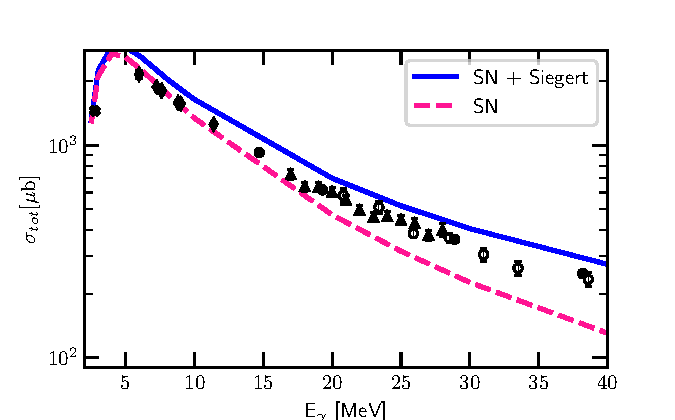
\includegraphics[width=0.75\textwidth]{Figures_De/TOTAL_CROSSSECTION_SMALL_REGION.pdf}
        \end{center}
        \caption{Total cross section as a function of the photon's energy E$_\gamma$.
        Solid blue line presents results obtained with SN+Siegert 
        and dashed pink line - with only SN current.
        The experimental data are from \cite{Bernabei1986} (black filled circles),
        \cite{BOSMAN1979} (empty circles),
        \cite{ARENDS1984} (squares),
        \cite{Skopik1974} (triangles),
        \cite{Moreh1989} (cross "X") and
        \cite{Birenbaum1985} (dimonds).
        }
        \label{TOTAL_CROSS_small}
    \end{figure}

    
    \begin{figure}[htb!]
        \begin{center}
        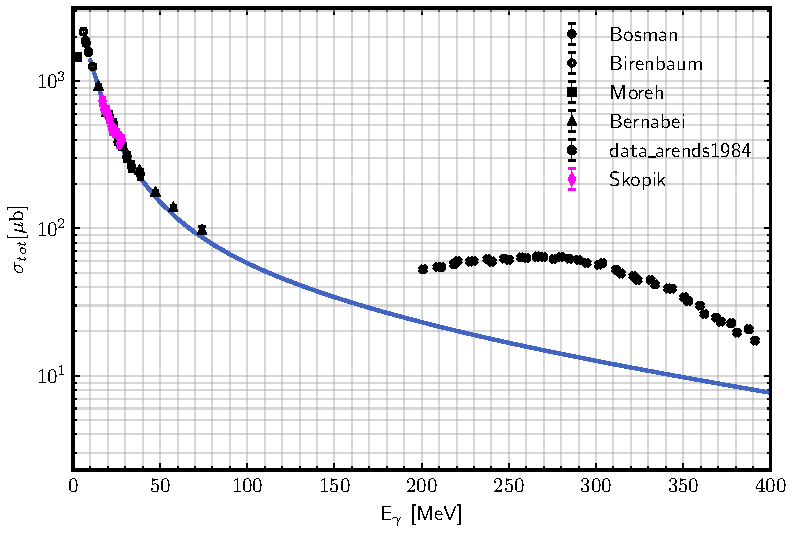
\includegraphics[width=0.75\textwidth]{Figures_De/TOTAL_CROSSSECTION.pdf}
        \end{center}
        \caption{The same as on the Fig.~\ref{TOTAL_CROSS} but for the energy range 2.5 - 400 MeV.
        }
        \label{TOTAL_CROSS}
    \end{figure}

    \begin{figure}[htb!]
        \begin{center}
            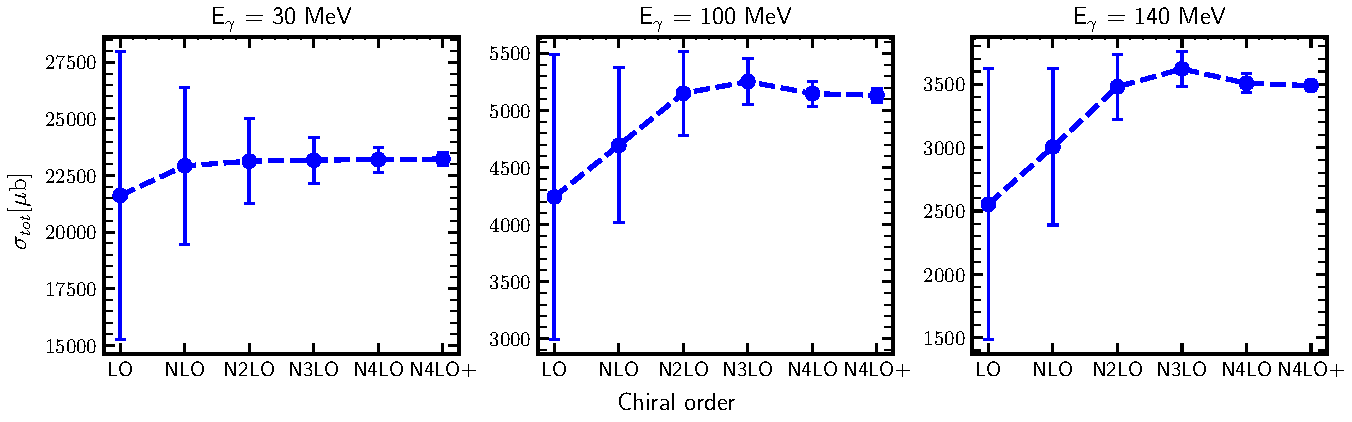
\includegraphics[width=0.95\textwidth]{Figures_De/TOTAL_CROSSSECTION_Truncation.pdf}
        \end{center}
        \caption{Total cross section of the deuteron photonisintegration
        process as a dependance on the chiral order for three photon energy E$_\gamma$ values: \SIlist[list-units = single]{30;100;140}{\mev}.
        Error bands show an estimated truncation error at each order.}
        \label{Trunc_100}
    \end{figure}
    
    In Fig. \ref{Trunc_100} I present 
    an example of such a procedure being applied to the
    total cross-section for the deuteron photodisintegration 
    at three photon energie values: \SIlist[list-units = single]{30;100;140}{\mev} as a function of the chiral order.
    Error bands show truncation errors calculated using Eq.~\ref{trunc2}~-~\ref{trunc5}.
    One can see that truncation errors are being reduced with each consecutive chiral order: for LO it is the biggest
    while for N4LO+ it is hardly visible at presented scale.
    In each case the prediction is within the uncertainty range of lower orders.
    
        
    Figures \ref{Diff_cross_order} - \ref{Diff_cross_err} show my predictions for the differential cross section
    $\frac{d\sigma}{d\Omega}$, where each subfigure 
    presents results obtained using different values of the photon energy:
    \SIlist[list-units = single]{30;100;140}{\mev}
    with 2N current's contributions taken into account via Siegert theorem. 
    % They all are organized in a similar way: the left panel
    % presents predictions obtained using \gls*{sms} potential at different chiral orders (from LO to N$^4$LO+)
    % with cutoff parameter $L = 450$~MeV,
    % the middle panel includes the truncation error's bands (described in Sec. \ref{sec:deut_bound})
    % for each chiral order starting
    % from NLO. And the right panel shows predictions obtained with different values of the
    % cutoff parameter at the chiral order N$^4$LO+.
    Fig.~\ref{Diff_cross_order} shows the predictions obtained using 
    different chiral orders (from LO to N$^4$LO+) and with $\Lambda=$~\SI{450}{\mev}.
    Comparing the best predictions (N$^4$LO+, $\Lambda=$~\SI{450}{\mev}) for each
    subfigure, we can
    conclude that the higher photon's energy is, the larger is 
    difference between the theoretical predictions and experimental 
    measurements. At $E_\gamma = $~\SI{30}{\mev} (top panel) my predictions
    almost perfectly match the data and the difference is almost always
    within the experimental uncertainties. Going to the energy \SI{100}{\mev} (middle subfigure)
    the descriptions seems not to be such good: theoretical
    predictions match the data qualitatively, but
    the gap in the angles range ($\ang{60} < \theta_p < \ang{130}$) 
    is around \SI{30}{\percent} ({\color{red} check the value!}).
    Looking at the bottom figure, it is even hard to say about 
    good qualitative description: the general trend of the
    angular dependance is presented, but still the predictions are 
    far from {\color{red} the ?} experimental values.

    Figures for each energy confirm the convergence 
    of the predictions with respect to the chiral order.
    We see that the curves at LO are far from both experimental 
    data and the best potential's predictions (N$^4$LO+) and
    the higher is photon's energy, the larger is this
    difference. With each subsequent chiral order, the 
    curves are more closer to each other and the difference
    between N$^4$LO and N$^4$LO+ is hardly visible at current scale.
    The relative difference at \SI{30}{\mev} around the point of maximum 
    ($\theta_p = \ang{80}$) is \SI{0.05}{\percent} which is \SI{0.02}{\micro \barn \per \steradian};
    at \SI{100}{\mev} and $\theta_p = \ang{107}$ it is \SI{0.79}{\percent} (\SI{0.025}{\micro \barn \per \steradian});
    and at \SI{140}{\mev} (same angle) it is 1.80\% - 0.043 \unit{\micro \barn \per \steradian}.
    Having such a small differences between predictions from two highest chiral orders,
    I can conclude that predictions are converged and 
    further chiral orders would rather not bring large contribution 
    to the cross section values. 
    The difference with experimental data is rather systematic 
    and is independent on the chiral order. 
    The relative difference between experimental data and predictions obtained with $N^4LO+$ and $\Lambda=$~\SI{450}{\mev} at \SI{30}{\mev} is less then \SI{13}{\percent}
    and absulute difference is < \SI{3.07}{\micro \barn \per \steradian}.
    At \SI{100}{\mev} descripancy is larger and relative difference reaches 46\% with absolute difference up to \SI{1.39}{\micro \barn \per \steradian}.
    Coming to \SI{140}{\mev} the relative difference 
    increases up to \SI{48.6}{\percent} and absolute - \SI{1.93}{\micro \barn \per \steradian}.
    What may be helpful
    for a better data description is a 2N current 
    and relativistic correction, mentioned earlier.

    Predictions obtained with \gls*{av18} potential (dashed-dotted purple line on the \fig{Diff_cross_order}) show that
    it is very similar at lower energies (relative difference at \SI{30}{\mev} is \SI{0.06}{\percent}
    at the point of maximum - \ang{80}) and with increasing energy to \SI{140}{\mev}
    it growes to \SI{3.1}{\percent]} at same angle. 
    It can be connected with our potential's quality loss, but \gls*{av18} can
    be struggling with high energies as well.

    The Fig.~\ref{Diff_cross_truncation} 
    presents theoretical truncation uncertainties and it once more
    confirms that for the regarded nuclear reaction chiral order
    N$^4$LO+ is able to produce converged predictions: 
    the black band is hardly visible for the $E_\gamma=$~\SI{30}{\mev}
    (the relative error for N$^4$LO+ at \ang{80} is only \SI{0.12}{\percent})
    and is also quite narrow for larger energies (at \SI{140}{\mev} 
    the error at the same angle is \SI{1.42}{\percent}). 

    Fig.~\ref{Diff_cross_cutoff} presents a cutoff dependency
    of predictions. The ideal case is when the dependency is so weak that
    the choice of the parameter $\Lambda$ would not make large 
    changes. In practice the choice of this parameter can be 
    important as it makes a noticeable difference in predictions.
    
    On the top of \fig{Diff_cross_cutoff} (when $E_\gamma=$~\SI{30}{\mev}) the cutoff dependance is so weak,
    that, in fact, all the lines (for different $\Lambda$ values)
    overlap each other and we cannot distinguish them with the naked eye:
    the relative difference ar maximum is \SI{0.08}{\percent}.
    Nevertheless, with increasing photon's energy to \SIlist{100; 140}{\mev} 
    (middle and bottom rows of \fig{Diff_cross_cutoff}) the spread becomes larger:
    the cutoff error is  \SI{3.35}{\percent} at \SI{100}{\mev}
    and \SI{5.56}{\percent} at \SI{140}{\mev} (the same $\theta_p$). 

    On the Fig.~\ref{Cutoff_dep} we saw that the total
    cross section for the same energies has the cutoff spread
    around \SI{4.5}{\percent} for \SI{100}{\mev} and \SI{8}{\percent} for \SI{140}{\mev}. For \SI{30}{\mev} it is below  \SI{1}{\percent}.
    
    In \fig{Diff_cross_pw_1nc} I show different components of the best prediction (N$^4$LO+, $\Lambda=\SI{450}{\mev}$)
    for three values of photon's energy. Prediction with plane-wave component only (without rescattering part)
    has relatively small deviation from the full predictions, but the difference increases at larger energies.
    With $E_\gamma=\SI{30}{\mev}$ the relative difference is \SI{10}{\percent} (\SI{4.03}{\micro \barn \per \steradian})
    at $\theta_p = \ang{80}$. Difference at \SI{100}{\mev} and the same angle is \SI{4}{\percent} (\SI{0.21}{\micro \barn \per \steradian})
    and at \SI{140}{\mev} it is \SI{7}{\percent} (\SI{0.21}{\micro \barn \per \steradian}).
    In contrast, predictions without Siegert component (1NC) have much larger gap with full prediction:
    the difference is \SI{46.5}{\percent} (\SI{13.67}{\micro \barn \per \steradian}) at \SI{30}{\mev},
    \SI{78.6}{\percent} (\SI{2.88}{\micro \barn \per \steradian}) at \SI{100}{\mev} and
    \SI{77.8}{\percent} (\SI{1.68}{\micro \barn \per \steradian}) at \SI{140}{\mev}.
    Obviously 2NC contributions are extremely important in this case, the difference connected with 2NC
    contributions is much higher then theoretical errors or even rescattering contribution.



    \begin{figure}[h]
        \centering
        \begin{subfigure}[t]{0.46\textwidth}
            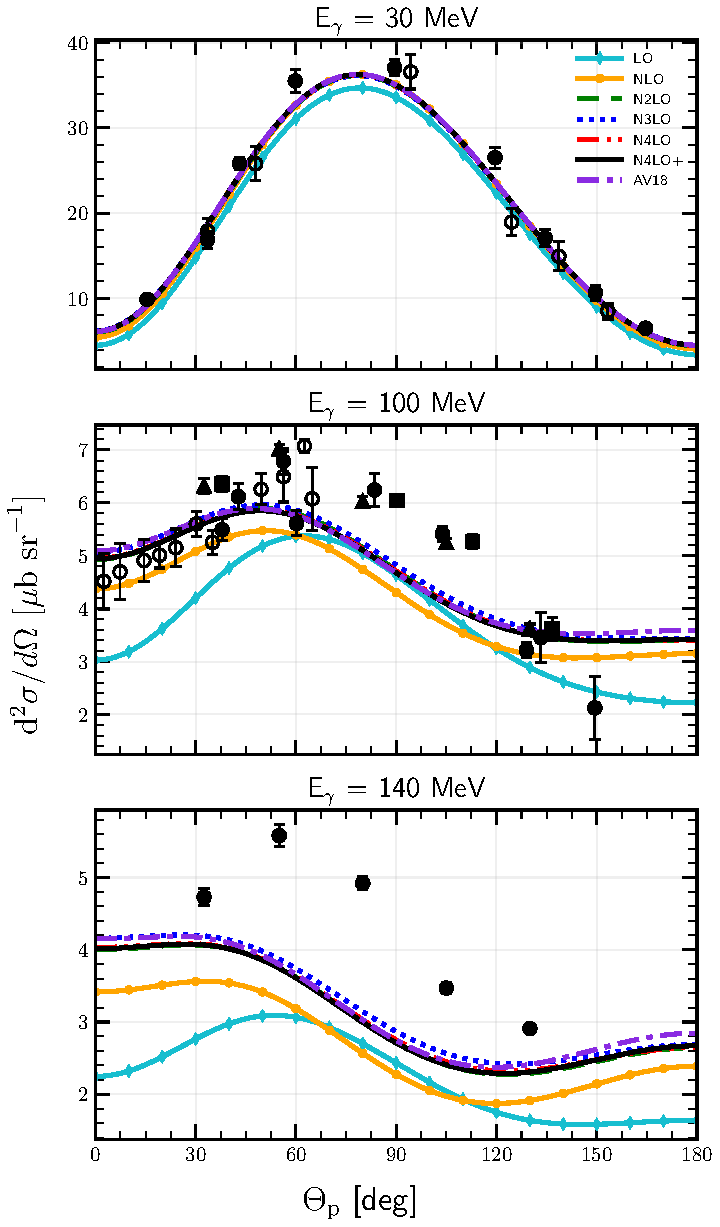
\includegraphics[width=\textwidth]{Figures_De/CROSS2_order_vert.pdf}
            \caption{}
            \label{Diff_cross_order}
        \end{subfigure}
        \begin{subfigure}[t]{0.46\textwidth}
            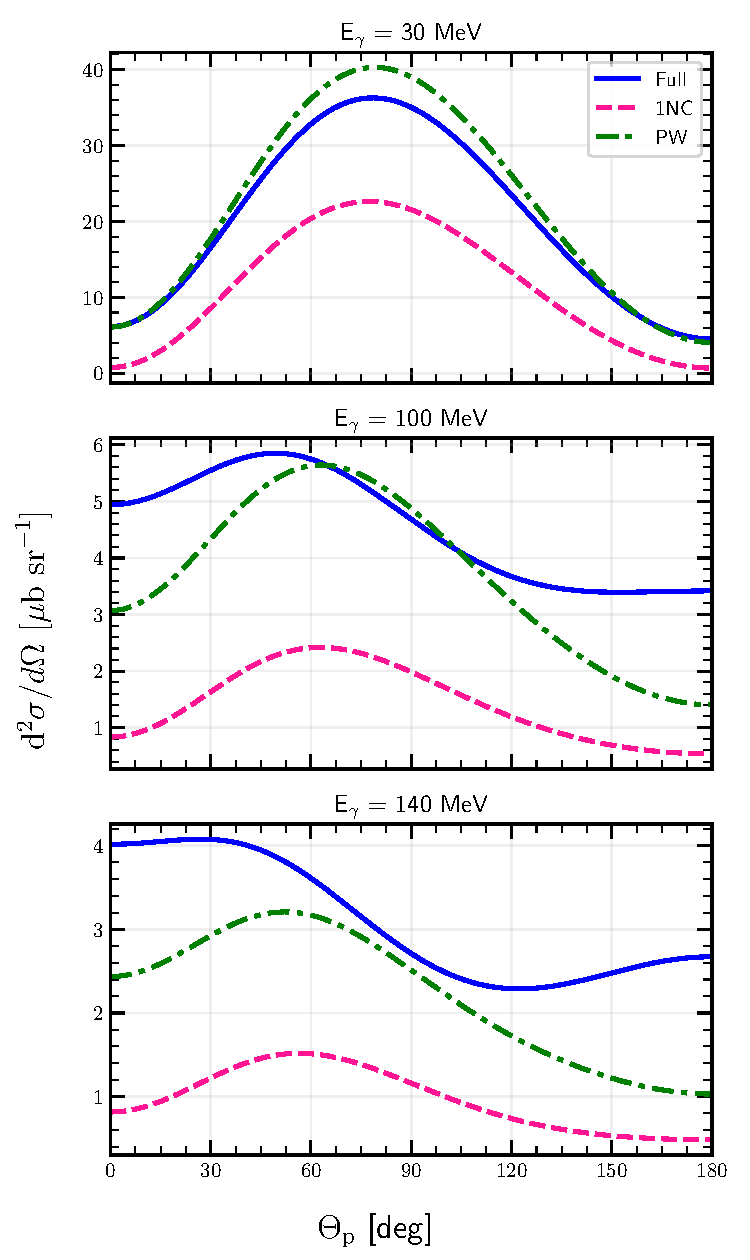
\includegraphics[width=\textwidth]{Figures_De/Diff_cross_pw_1nc.pdf}
            \caption{}
            \label{Diff_cross_pw_1nc}
        \end{subfigure}
        \caption{Differential cross section as a function of the outgoing proton angle in the center of mass frame 
        for the photon's energy \SI{30}{\mev} (top), \SI{100}{\mev} (middle) and \SI{140}{\mev} (bottom).
        {\bf (a)} Results obtained using \gls*{sms} potential
        at different chiral orders (from LO to N$^4$LO+) with the cutoff parameter $\Lambda=450$~MeV and 
        2NC contributions taking via Siegert theorem.
        For the sake of comparison, predictions obtained with the \gls*{av18} potential are on both figures as well.
        Data points (filled and empty circles) are from \cite{Ying_Experiment_Deut}
        for $E_\gamma=\SIlist[list-units = single]{30; 100}{\mev}$
        and \cite{DeSanctis_Experiment_Deut} for $E_\gamma=\SI{140}{\mev}$.
        {\bf (b)} Predictions obtained with chiral N$^4$LO+ potential and $\Lambda=\SI{450}{\mev}$ are on {\bf (b)}.
        Blue solid line is a best predictions we have (plane-wave plus rescattering parts, 1NC + Siegert), pink dashed line shows predictions obtained with
        single-nucleon current only (without Siegert contributions) and green dashed-dotted line
        is a prediction with plane-wave part only - without rescattering.
        }
        % Results in {\bf (a)} are obtained using \gls*{sms} potential
        % at different chiral orders (from LO to N$^4$LO+) with the cutoff parameter $\Lambda=450$~MeV and 
        % 2NC contributions taking via Siegert theorem.
        % Data points (filled and empty circles) are from \cite{Ying_Experiment_Deut}
        % for (\SIlist[list-units = single]{30; 100}{\mev})
        % and \cite{DeSanctis_Experiment_Deut} (for energy \SI{140}{\mev}).
        % Predictions obtained with chiral N$^4$LO+ potential and $\Lambda=\SI{450}{\mev}$ are on {\bf (b)}.
        % Blue solid line is a best predictions we have (plane-wave plus rescattering parts, 1NC + Siegert), pink dashed line shows predictions obtained with
        % single-nucleon current only (without Siegert contributions) and green dashed-dotted line
        % is a prediction with plane-wave part only - without rescattering.}
        \label{Diff_cross_order_pw}
    \end{figure}


        
    \begin{figure}[h]
        \centering
        \begin{subfigure}[t]{0.46\textwidth}
            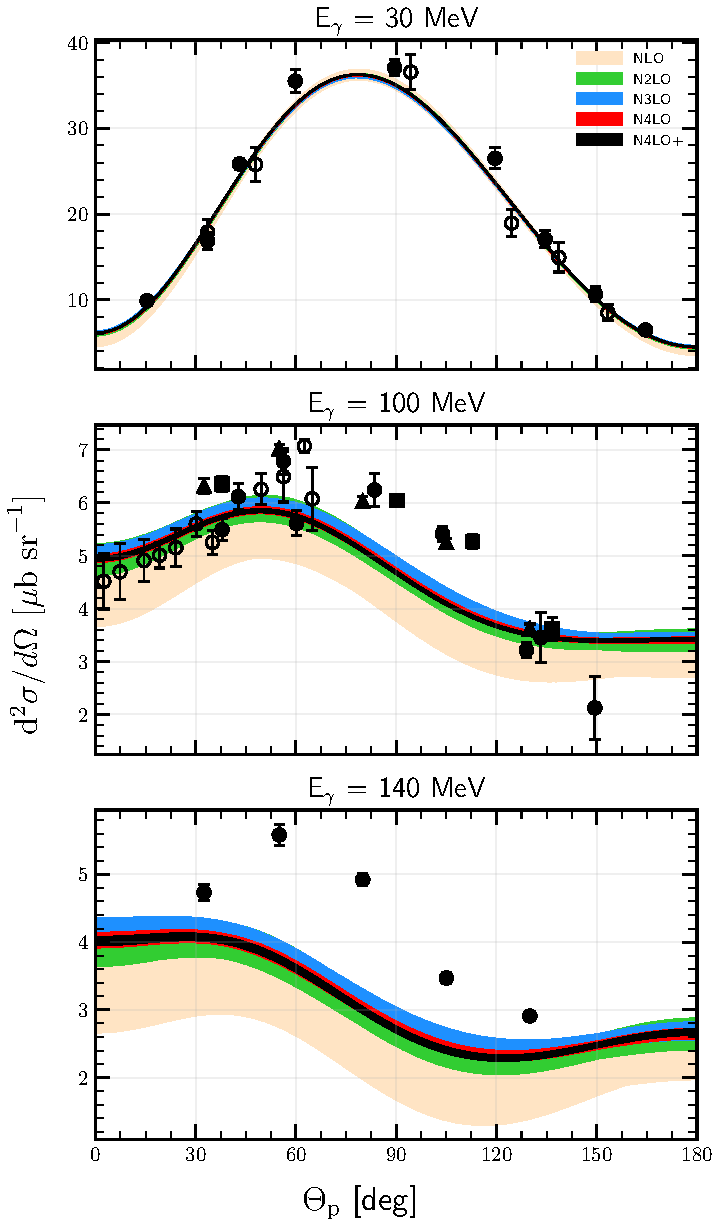
\includegraphics[width=\textwidth]{Figures_De/CROSS2_truncation_vert.pdf}
            \caption{ Truncation error bands.}
            \label{Diff_cross_truncation}
        \end{subfigure}
        \begin{subfigure}[t]{0.46\textwidth}
            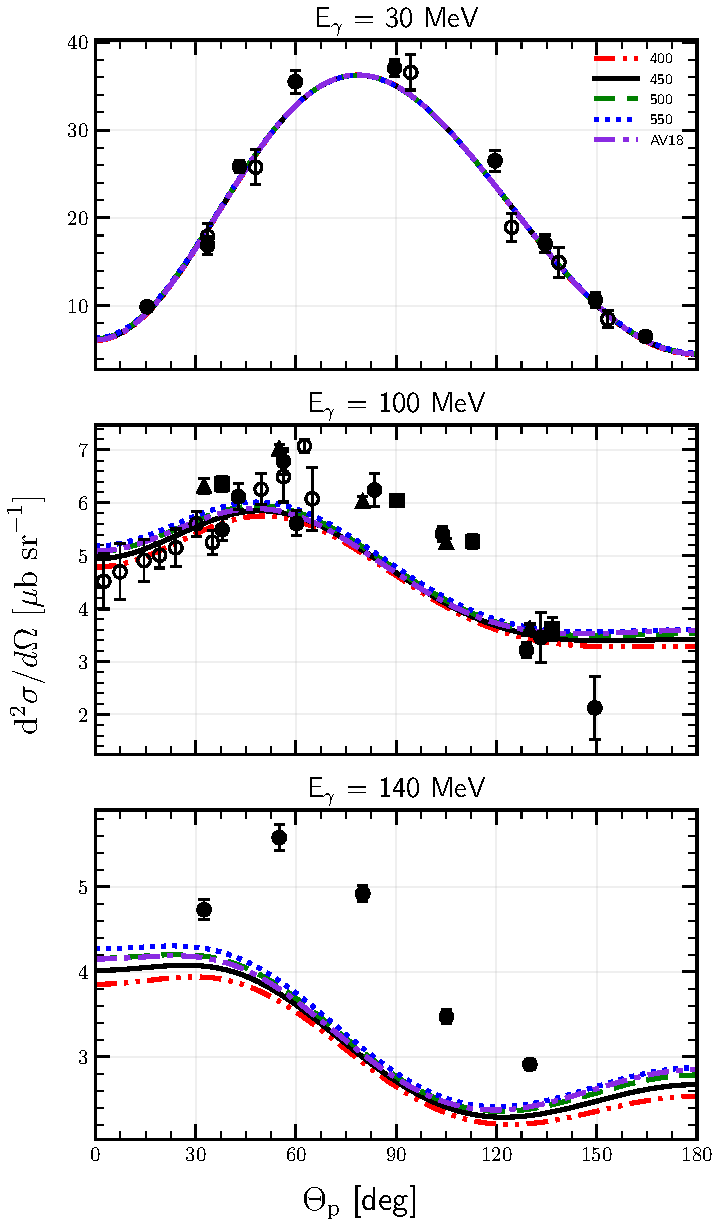
\includegraphics[width=\textwidth]{Figures_De/CROSS2_cutoff_vert.pdf}
            \caption{Cutoff dependance  of predictions.}
            \label{Diff_cross_cutoff}
        \end{subfigure}
        \caption{Theoretical uncertainies 
        for the differential cross section $\frac{d^2\sigma}{d\Omega}$
        as a function of the outgoing proton's momentum polar angle $\theta_p$ in the center of mass frame 
        for the photon's energy is \SI{30}{\mev} (top row), \SI{100}{\mev} (middle row) and \SI{140}{\mev} (bottom row).
        Figure {\bf(a)} presents the truncation error bands for each energy in a corresponding row. 
        Results are obtained using potential with different chiral orders (from NLO to N$^4$LO+) 
        with cutoff parameter $\Lambda=\SI{450}{\mev}$ and 2NC contributions taking via Siegert approach.
        Figure {\bf (b)} shows predictions obtained using different values of the cutoff parameter $\Lambda$
        (double-dotted-dashed red line presents results obtaining with 
        a cutoff values $\Lambda=\SI{400}{\mev}$, solid black line - \SI{450}{\mev}, dashed green line - \SI{500}{\mev}
        and dotted blues line - \SI{550}{\mev}) and the chiral potential N$^4$LO+. 
        Data points (filled and empty circles) are from \cite{Ying_Experiment_Deut}
        for $E_\gamma=\SIlist[list-units = single]{30; 100}{\mev}$
        and from \cite{DeSanctis_Experiment_Deut} for $E_\gamma=\SI{140}{\mev}$.}
        \label{Diff_cross_err}
    \end{figure}

    \clearpage

    \subsection{Polarisation observables}
    \label{tensor_results}

    In this subsection I will present my predictions for 
    selected polarisation observables.
    I start with deuteron analyzing power $T_{20}$, $T_{21}$ and $T_{22}$,
    which according to \cite{ArenhovelPhotodisint1991} are defined as:
    
    \begin{equation}
        T_{2i} (\theta) = \frac{(2 - \delta_{i0}) \Re V_{2i}}{V_{00}}, i=0,1,2
    \end{equation}

    On the Figures \ref{T20_T21_30} (a, b) and \ref{T22_T11_30}(a,b)
    I show my predictions for the
    $T_{20}$, $T_{21}$,  and $iT_{11}$ respectively as a functions 
    of the outgoing proton angle $\theta$ in the CM frame. Each of them
    is prepared with photon's energy 30~MeV and is
    organized in the similar way: the top
    pane shows a dependance of the predictions on the 
    chiral order of the potentia. The middle subfigure is
    showing a correspondent truncation error for each of the 
    predictions from a top one (without LO, because its uncertainty is
    too large and will make the readability worse). The last (bottom)
    pane shows the cutoff dependance for each observable at the chiral
    order N$^4$LO+. 

    All the polarisation observables presented here, show a good convergence 
    upon a chiral order as it is hard to distinguish the predictions
    from each subsequent order starting from the N$^2$LO. 
    The slowest convergence is observed for $iT_{11}$ (Fig.~\ref{T11_30_vert})
    where we can stll recognize N$^2$LO band.
    The cutoff dependency for all regarded observables is weak and 
    predictions for each value of the $\Lambda$ are hardly separable 
    with the naked eye. 


    Predictions for the photon's energy $E_\gamma = 100$~MeV
    (Figs. \ref{T20_T21_100} and \ref{T22_T11_100}) preserve similar
    trends for each obserable. 
    Generally, predictions are being converged starting
    even from the N$^2$LO while for $iT_{11}$
    we can see 
    that truncation error's bands are noticeably wide
    even at N$^4$LO and N$^4$LO+
    Cutoff dependance at this energy is a bit stronger, especially
    for 
    $T_{22}$ and $iT_{11}$ components (Fig.~\ref{T22_T11_30}),
    where one can see 
    slightly stronger discrepancy at the stationary points.
    
    Looking at the predictions for the deuteron tensor analyzing power,
    we can conclude that cutoff dependence is generally weak
    and the choice of $\Lambda$ does not affect predictions much.
    In the case of dependance on the chiral order, we can
    also see that predictions are mostly converged after N$^2$LO or N$^3$LO.
    One exception here is $iT_{11}$ which seem to be more sensitive
    to the choice of cutoff parameter and to the chiral order.
    This observable can be usefull for the investigation of global 
    convergence with respect to the chiral order and
    can indicate some problems in the model used for the
    deuteron photodisintegration.
    Of course, we can also confirm once more that 
    our model is less accurate at higher energies which is reflected
    in a stronger cutoff dependance and slower chiral convergence.


    \begin{figure}[htb]
        \centering
        \begin{subfigure}[b]{0.46\textwidth}
            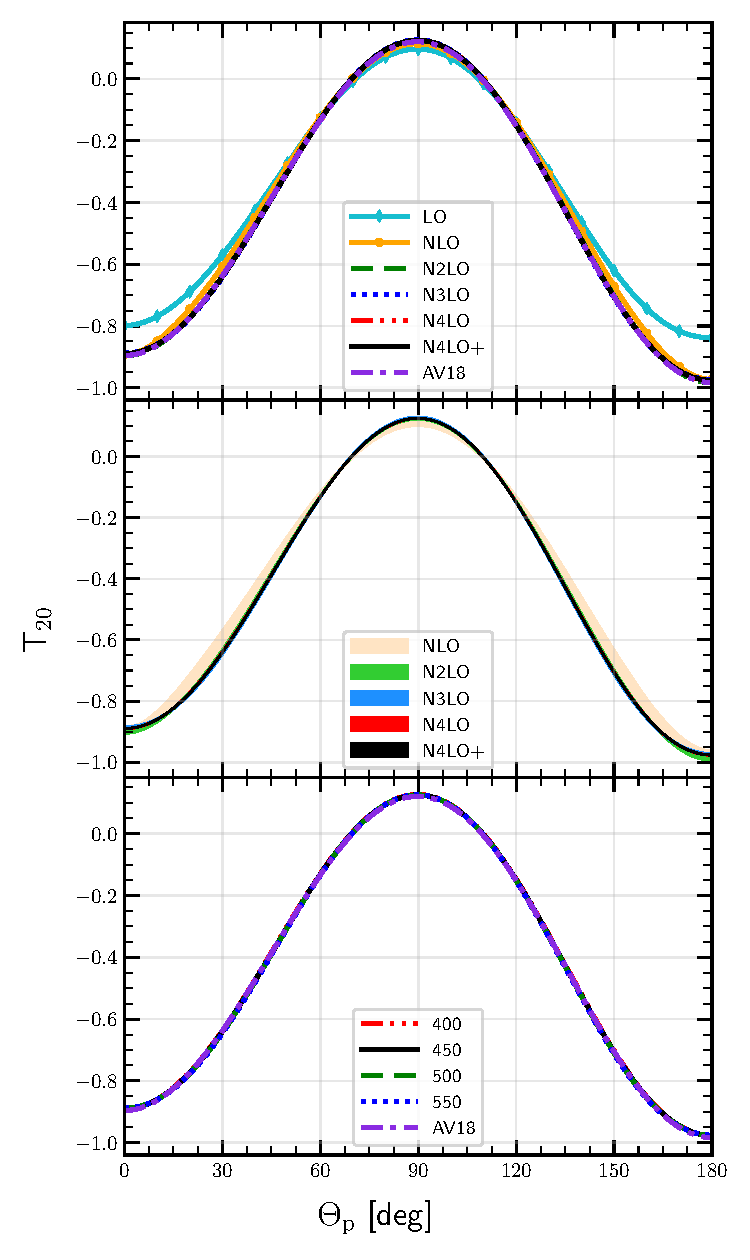
\includegraphics[width=\textwidth]{Figures_De/T20D2_30mev.pdf}
            \caption{T$_{20}$}
            \label{T20_30_vert}
        \end{subfigure}
        \begin{subfigure}[b]{0.46\textwidth}
            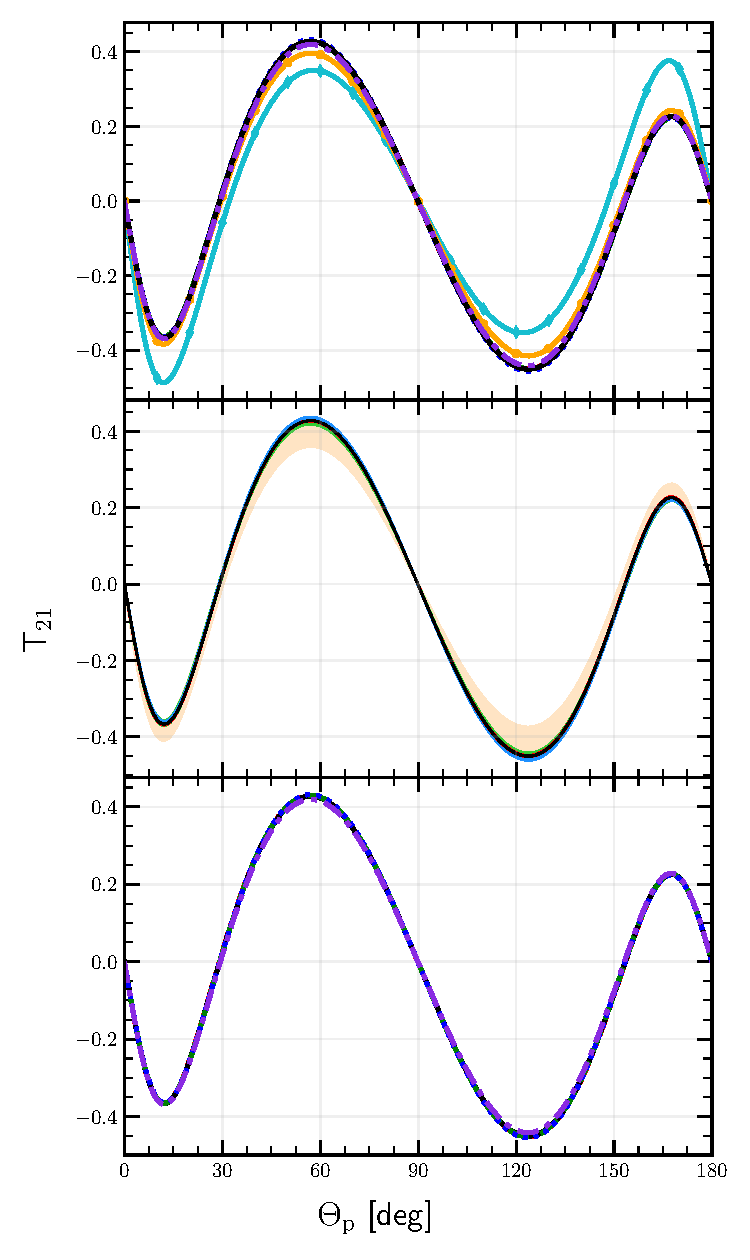
\includegraphics[width=\textwidth]{Figures_De/T21D2_30mev.pdf}
            \caption{T$_{21}$}
            \label{T21_30_vert}
        \end{subfigure}
        \caption{Tensor analyzing power T$_{20}$  {\bf (a)}
        and T$_{21}$ {\bf (b)}
        as a function of the outgoing proton angle in the center of mass frame 
        for the photon's energy \SI{30}{\mev}.
        Top row presents results obtained using potential
        with different chiral orders (from LO to N$^4$LO+) with cutoff parameter $\Lambda=450$~MeV.
        The middle row shows truncation errors for each 
        chiral order starting from NLO and
        bottom row presents a cutoff dependency (chiral potential N$^4$LO+).
        For the sake of comparison, predictions obtained with \gls*{av18} potential are on figures as well.}
        \label{T20_T21_30}
    \end{figure}

    \begin{figure}[htb]
        \centering
        \begin{subfigure}[b]{0.46\textwidth}
            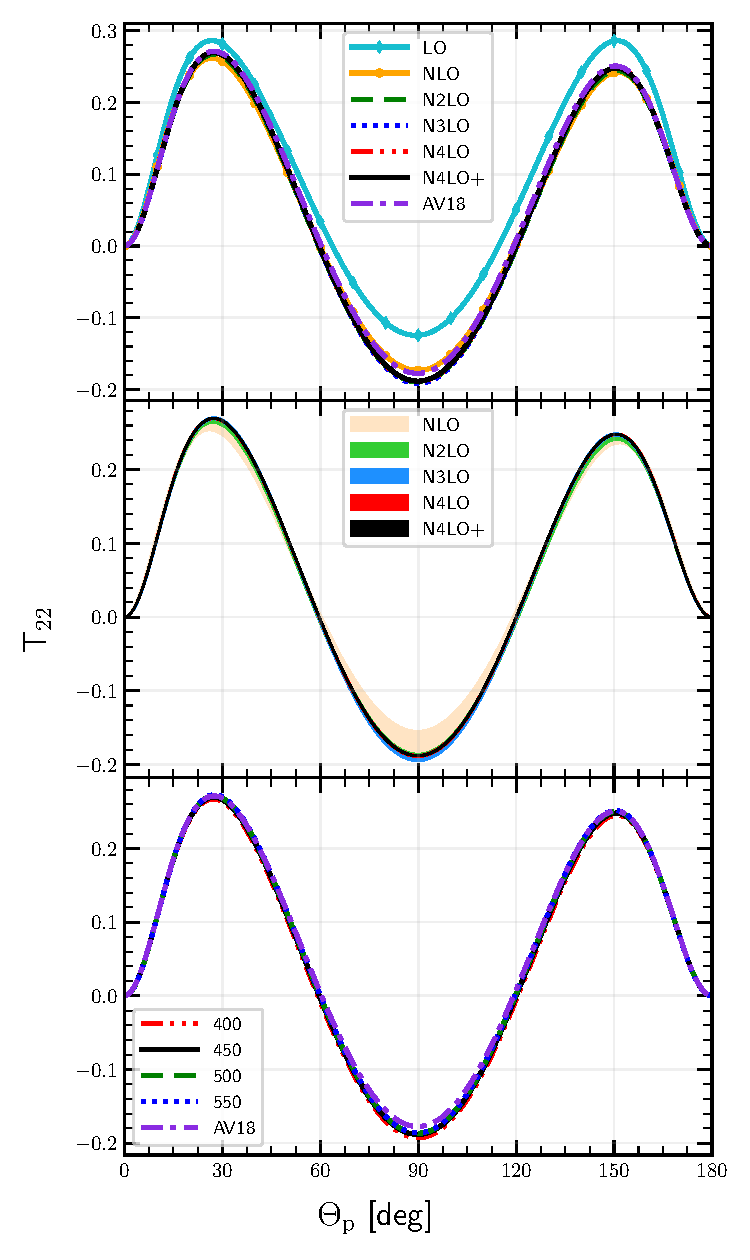
\includegraphics[width=\textwidth]{Figures_De/T22D2_30mev.pdf}
            \caption{T$_{22}$}
            \label{T22_30_vert}
        \end{subfigure}
        \begin{subfigure}[b]{0.46\textwidth}
            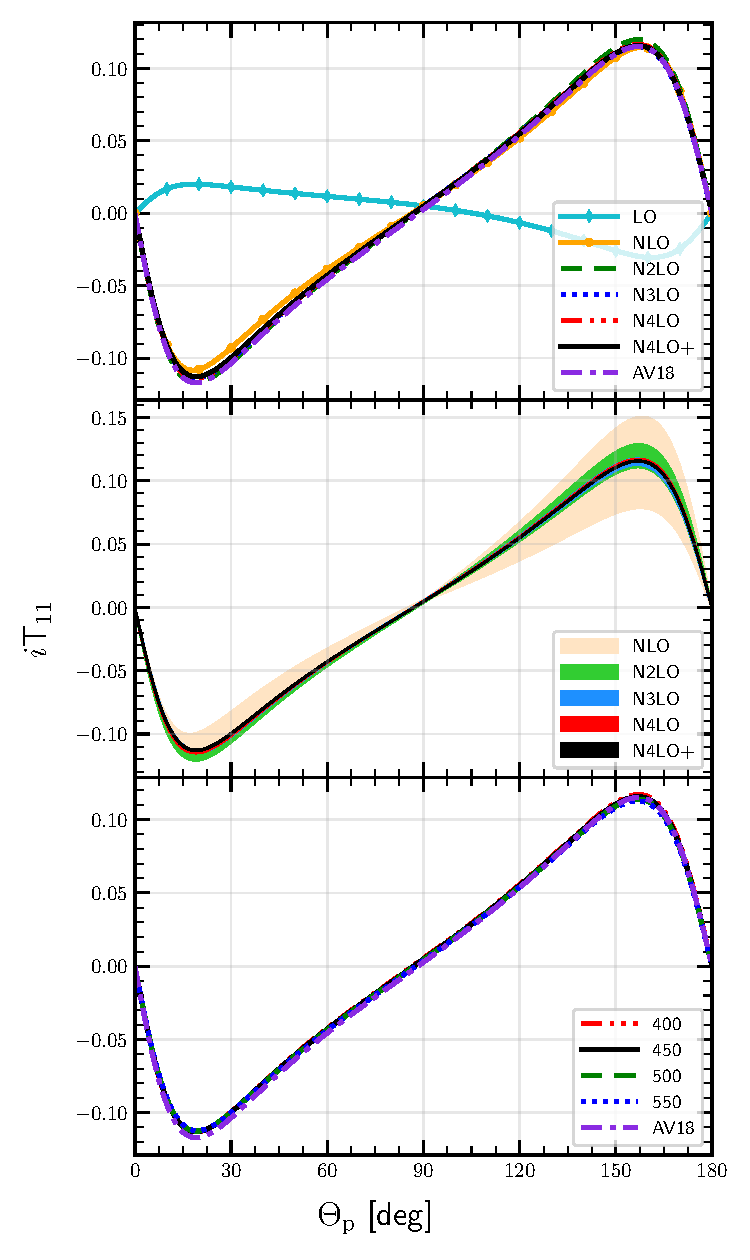
\includegraphics[width=\textwidth]{Figures_De/T11D2_30mev.pdf}
            \caption{iT$_{11}$}
            \label{T11_30_vert}
        \end{subfigure}
        \caption{The same as on \ref{T20_T21_30} but for polarisation observables
        T$_{22}$ (subfigure {\bf (a)}) and iT$_{11}$ (subfigure {\bf (b)}).}
        \label{T22_T11_30}
    \end{figure}

    \begin{figure}[htb]
        \centering
        \begin{subfigure}[b]{0.46\textwidth}
            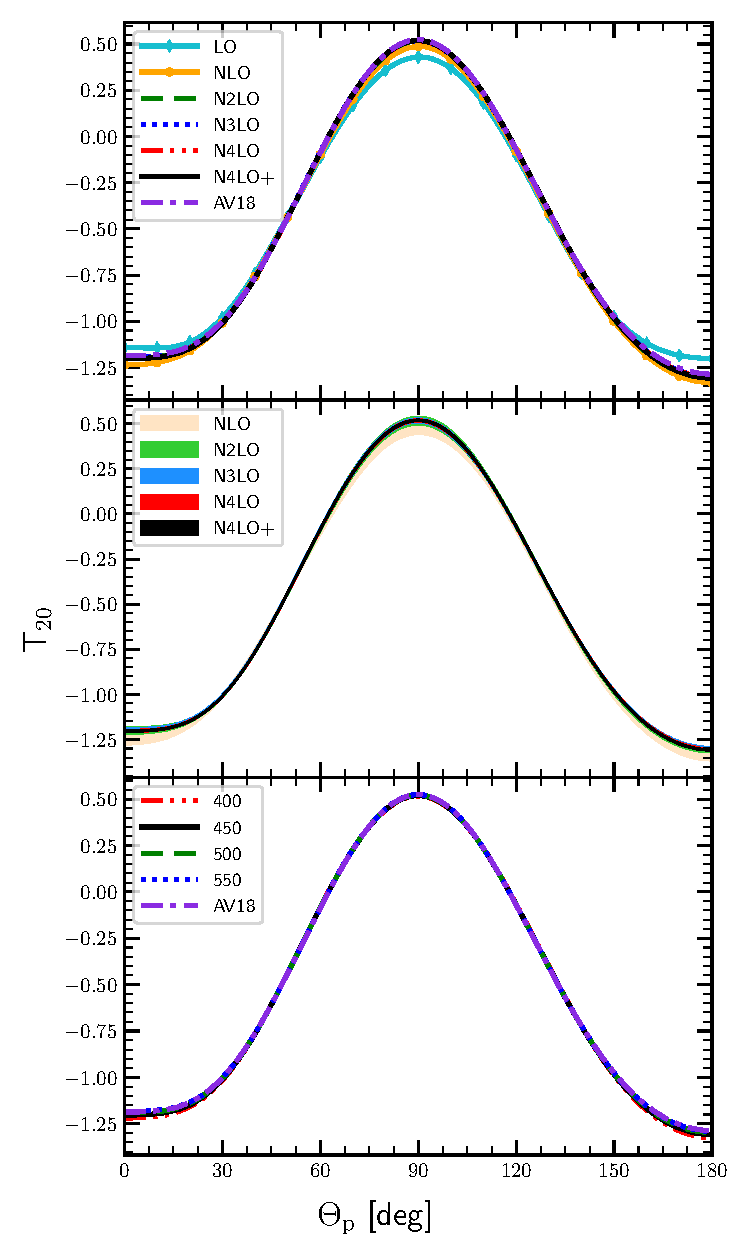
\includegraphics[width=\textwidth]{Figures_De/T20D2_100mev.pdf}
            \caption{T$_{20}$}
            \label{T20_100_vert}
        \end{subfigure}
        \begin{subfigure}[b]{0.46\textwidth}
            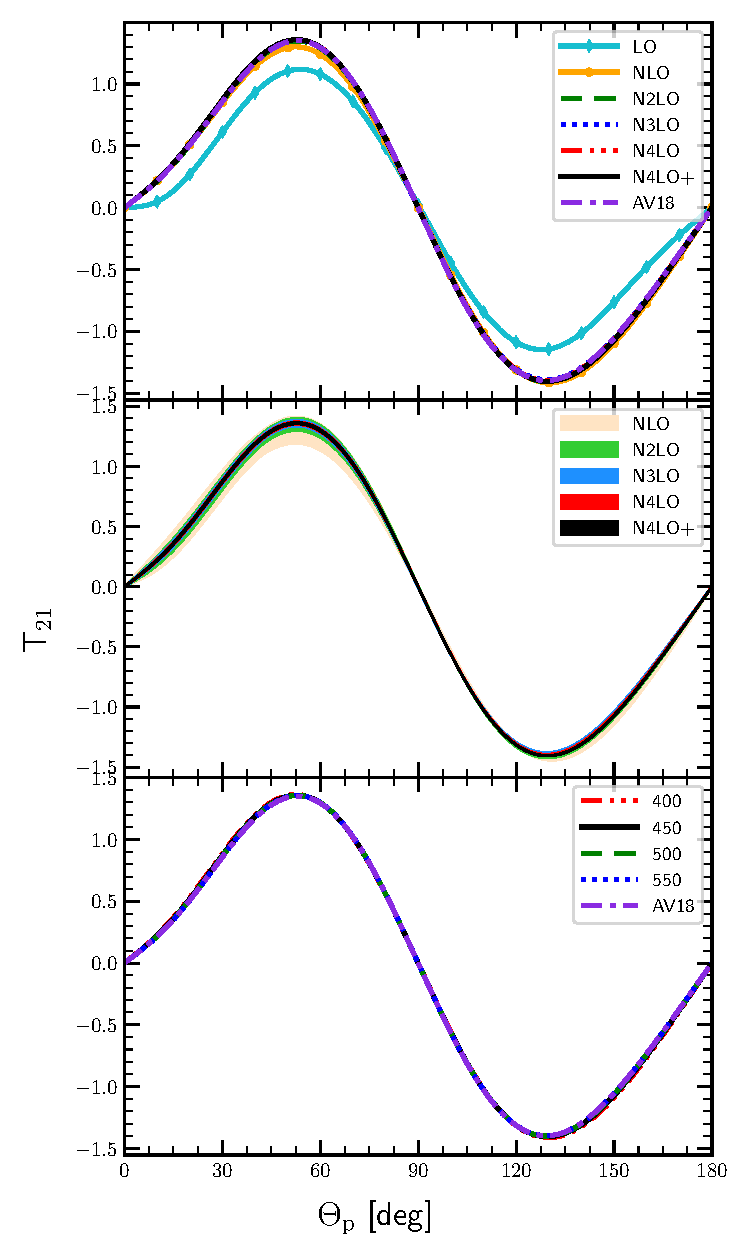
\includegraphics[width=\textwidth]{Figures_De/T21D2_100mev.pdf}
            \caption{T$_{21}$}
            \label{T21_100_vert}
        \end{subfigure}
        \caption{Tensor analyzing power T$_{20}$  {\bf (a)}
        and T$_{21}$ {\bf (b)}
        as a function of the outgoing proton angle in the center of mass frame 
        for the photon's energy \SI{100}{\mev}.
        Top row presents results obtained using potential
        with different chiral orders (from LO to N$^4$LO+) with cutoff parameter $\Lambda=450$~MeV.
        The middle row shows truncation errors for each 
        chiral order starting from NLO and
        bottom row presents a cutoff dependency (chiral potential N$^4$LO+).
        For the sake of comparison, predictions obtained with \gls*{av18} potential are on figures as well.}
        \label{T20_T21_100}
    \end{figure}

    \begin{figure}[htb]
        \centering
        \begin{subfigure}[b]{0.46\textwidth}
            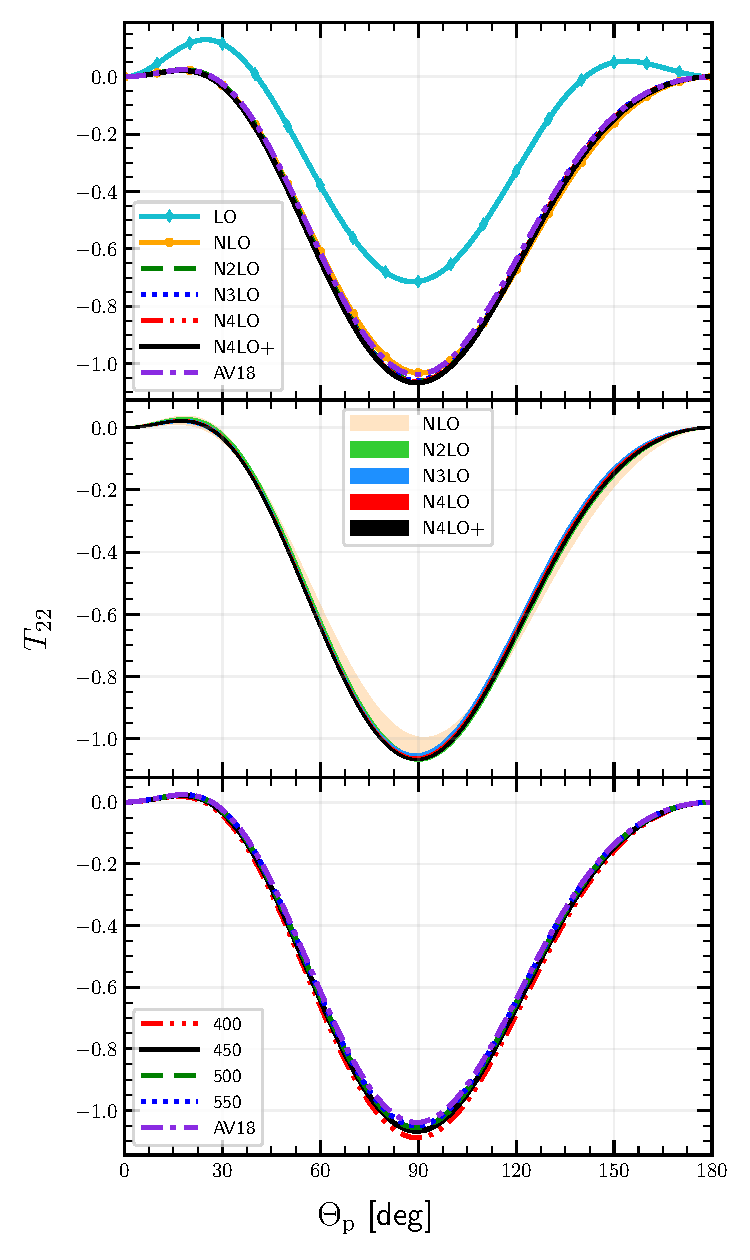
\includegraphics[width=\textwidth]{Figures_De/T22D2_100mev.pdf}
            \caption{T$_{22}$}
            \label{T22_100_vert}
        \end{subfigure}
        \begin{subfigure}[b]{0.46\textwidth}
            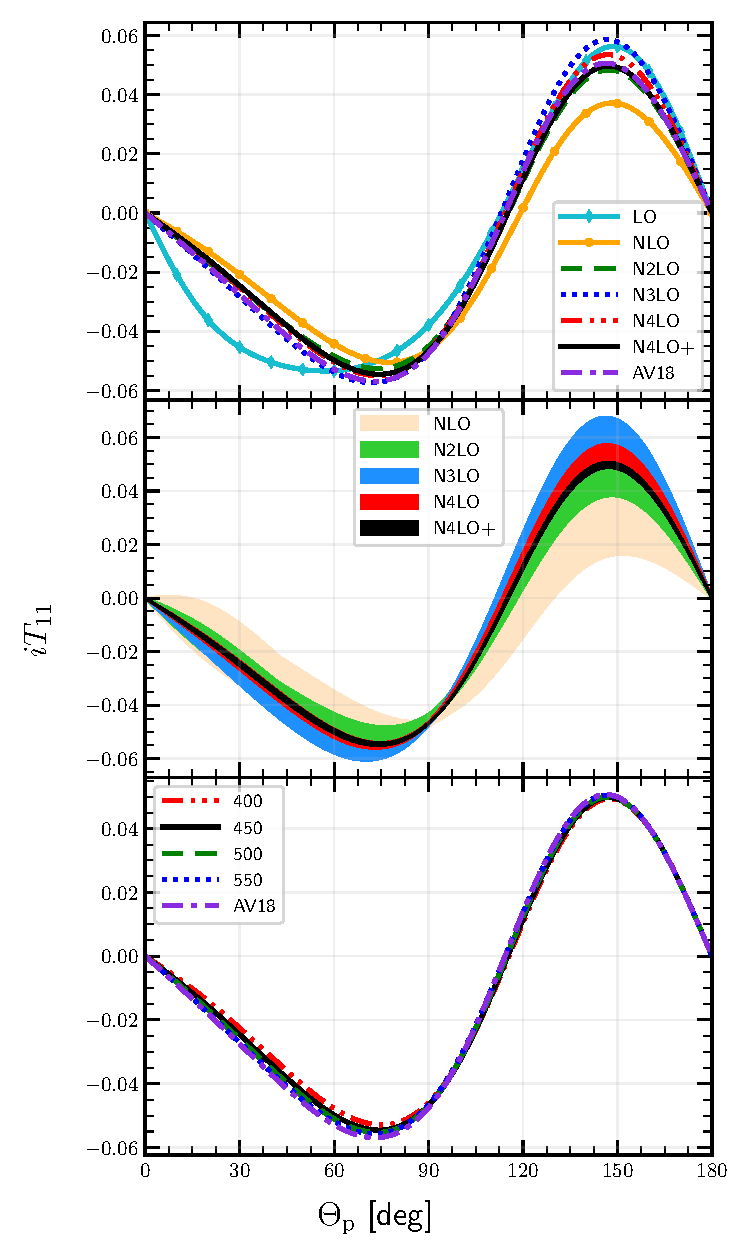
\includegraphics[width=\textwidth]{Figures_De/T11D2_100mev.pdf}
            \caption{iT$_{11}$}
            \label{T11_100_vert}
        \end{subfigure}
        \caption{The same as on \ref{T20_T21_100} but for polarisation observables
        T$_{22}$ (subfigure {\bf (a)}) and iT$_{11}$ (subfigure {\bf (b)}).}
        \label{T22_T11_100}
    \end{figure}

    \begin{figure}[h]
        \begin{center}
        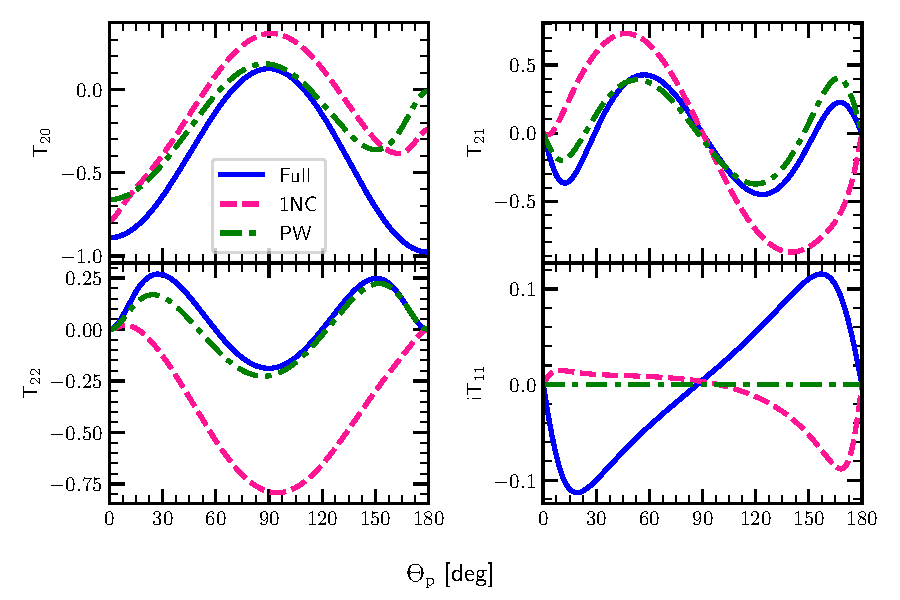
\includegraphics[width=0.9\textwidth]{Figures_De/TensorPowers_pw_1nc.pdf}
        \end{center}
        \caption{Tensor analyzing powers T$_{20}$, T$_{21}$ and T$_{22}$ as a functions of the
        outgoing proton angle $\theta_p$ (in the center of mass frame).
        Solid blue line is a mean value of my predictions obtained with a
        \gls*{sms} potential at N$^4$LO+ chiral order and with $\Lambda$~=~450~MeV
        at energy values from \SIrange[range-phrase=\text{ to }]{25}{45}{\mev} and
        where SN current was used together with Siegert approach. 
        Pink dashed line is similar prediction but with SN only. 
        The corresponding bands show the deviation of predictions in the regarded
        energy region.
        % Filled bands show maximal spread of my predictions obtained with a 
        % \gls*{sms} potential at N$^4$LO+ chiral order and with $\Lambda$~=~450~MeV
        % for the energy span from 25 to 45 MeV. Blue bands correspond to the
        % case where SN current was used together with Siegert approach and 
        % pink bands - to the SN currentonly. 
        Filled circles are experimental data
        from \cite{rachek2007} for the analogous energy span.}
        \label{tensor_angular_25-45}
    \end{figure}


    
    On the next figures, I show the predictions in a similar way as it was done
    in \cite{rachek2007} in order to compare my predictions with the experimental
    data. On the Figures \ref{tensor_angular_25-45} - \ref{tensor_angular_230-330}
    I show an angular dependance of the $T_{2i}$ ($i=0,1,2$) for a specific energy bands.
    Solid blue line shows an average value of the observable in the specified energy range
    obtained at N$^4$LO+ with $\Lambda=450$~MeV, while the pink dashed line is a prediction
    obtained with a same setup but without using a contributions from Siegert approach
    (single nucleon current only). Bands for each of prediction specify the spread of
    predictions in regarded energy band.
    
    One can see that the data description is better for the predictions with Siegert contributions 
    and SN current is not able to describe experiment properly. With increasing energy 
    (more than \SI{100}{\mev}),
    the difference between predicted values and experimental data becomes larger
    (especially for $T_{22}$), but the model I use is not meant to be used for high energies 
    and figures are presented out of the curiosity. 
    




    \begin{figure}[h]
        \begin{center}
        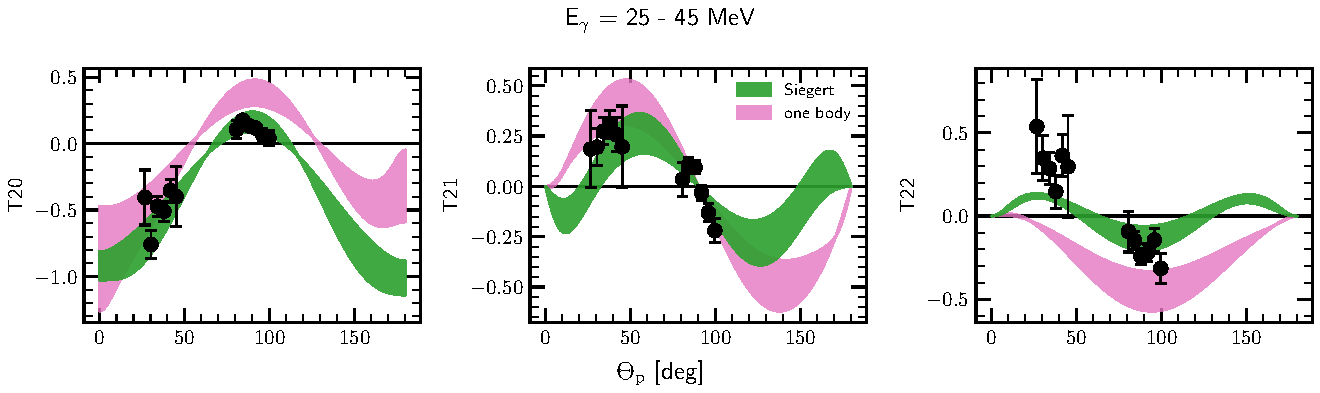
\includegraphics[width=1\textwidth]{Figures_De/Tensor_analyzing_power_angular_E25-45.pdf}
        \end{center}
        \caption{Tensor analyzing powers T$_{20}$, T$_{21}$ and T$_{22}$ as a functions of the
        outgoing proton angle $\theta_p$ (in the center of mass frame).
        Solid blue line is a mean value of my predictions obtained with a
        \gls*{sms} potential at N$^4$LO+ chiral order and with $\Lambda$~=~450~MeV
        at energy values from \SIrange[range-phrase=\text{ to }]{25}{45}{\mev} and
        where SN current was used together with Siegert approach. 
        Pink dashed line is similar prediction but with SN only. 
        The corresponding bands show the deviation of predictions in the regarded
        energy region.
        % Filled bands show maximal spread of my predictions obtained with a 
        % \gls*{sms} potential at N$^4$LO+ chiral order and with $\Lambda$~=~450~MeV
        % for the energy span from 25 to 45 MeV. Blue bands correspond to the
        % case where SN current was used together with Siegert approach and 
        % pink bands - to the SN currentonly. 
        Filled circles are experimental data
        from \cite{rachek2007} for the analogous energy span.}
        \label{tensor_angular_25-45}
    \end{figure}

    \begin{figure}[h]
        \begin{center}
        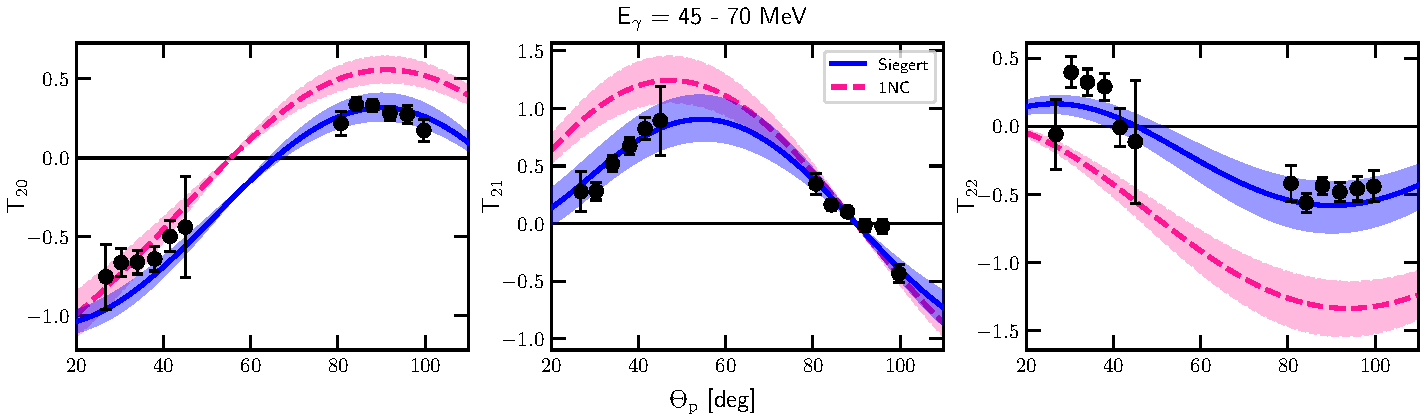
\includegraphics[width=0.95\textwidth]{Figures_De/Tensor_analyzing_power_angular_E45-70.pdf}
        \end{center}
        \caption{The same as on the Fig.~\ref*{tensor_angular_25-45} but for energy bin \SIrange{45}{70}{\mev}}
        \label{tensor_angular_45-70}
    \end{figure}

    \begin{figure}[h]
        \begin{center}
        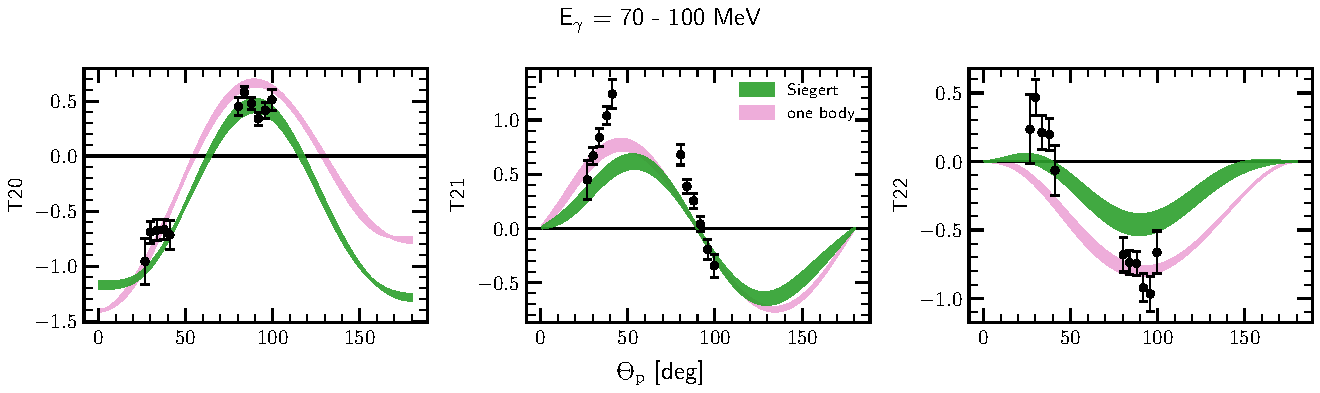
\includegraphics[width=0.95\textwidth]{Figures_De/Tensor_analyzing_power_angular_E70-100.pdf}
        \end{center}
        \caption{The same as on the Fig.~\ref*{tensor_angular_25-45} but for energy bin \SIrange{70}{100}{\mev}}
        \label{tensor_angular_70-100}
    \end{figure}        

    \begin{figure}[h]
        \begin{center}
        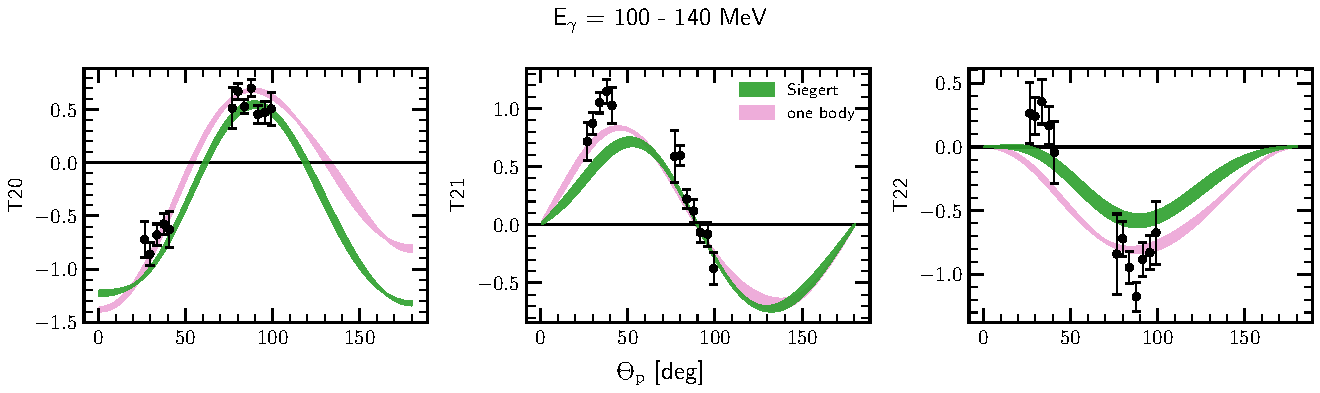
\includegraphics[width=0.95\textwidth]{Figures_De/Tensor_analyzing_power_angular_E100-140.pdf}
        \end{center}
        \caption{The same as on the Fig.~\ref*{tensor_angular_25-45} but for energy bin \SIrange{100}{140}{\mev}}
        \label{tensor_angular_100-140}
    \end{figure}
        
        

    \begin{figure}[h]
        \begin{center}
        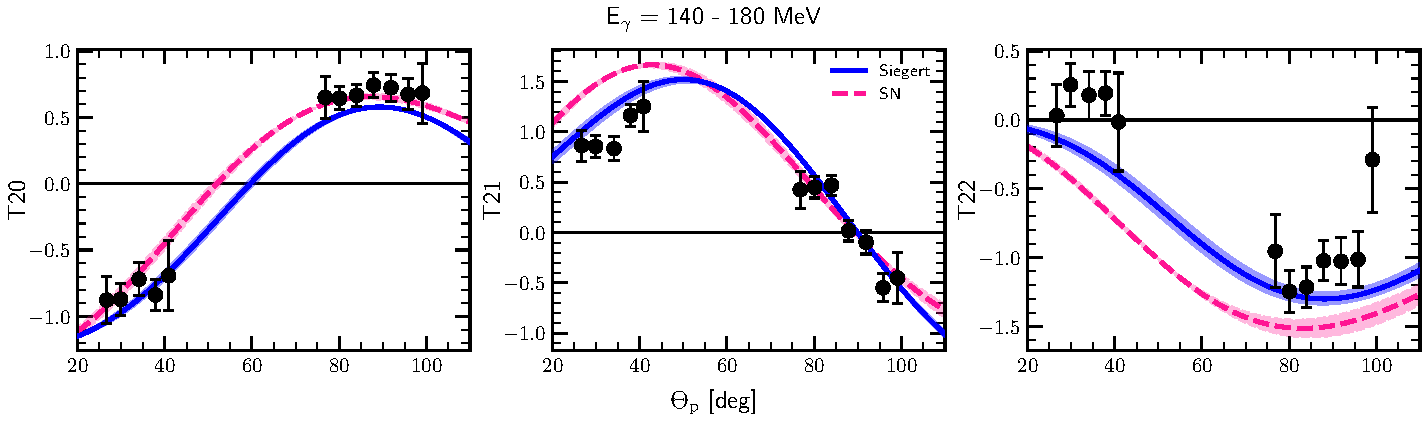
\includegraphics[width=0.95\textwidth]{Figures_De/Tensor_analyzing_power_angular_E140-180.pdf}
        \end{center}
        \caption{The same as on the Fig.~\ref*{tensor_angular_25-45} but for energy bin \SIrange{140}{180}{\mev}}
        \label{tensor_angular_140-180}
    \end{figure}
        

    \begin{figure}[h]
        \begin{center}
        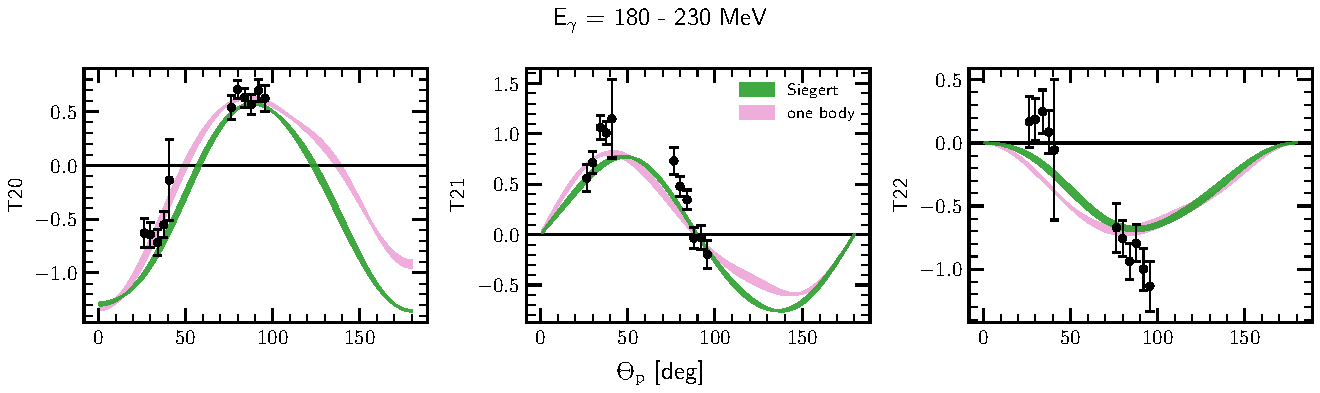
\includegraphics[width=0.95\textwidth]{Figures_De/Tensor_analyzing_power_angular_E180-230.pdf}
        \end{center}
        \caption{The same as on the Fig.~\ref*{tensor_angular_25-45} but for energy bin \SIrange{180}{230}{\mev}}
        \label{tensor_angular_180-230}
    \end{figure}

    \begin{figure}[h]
        \begin{center}
        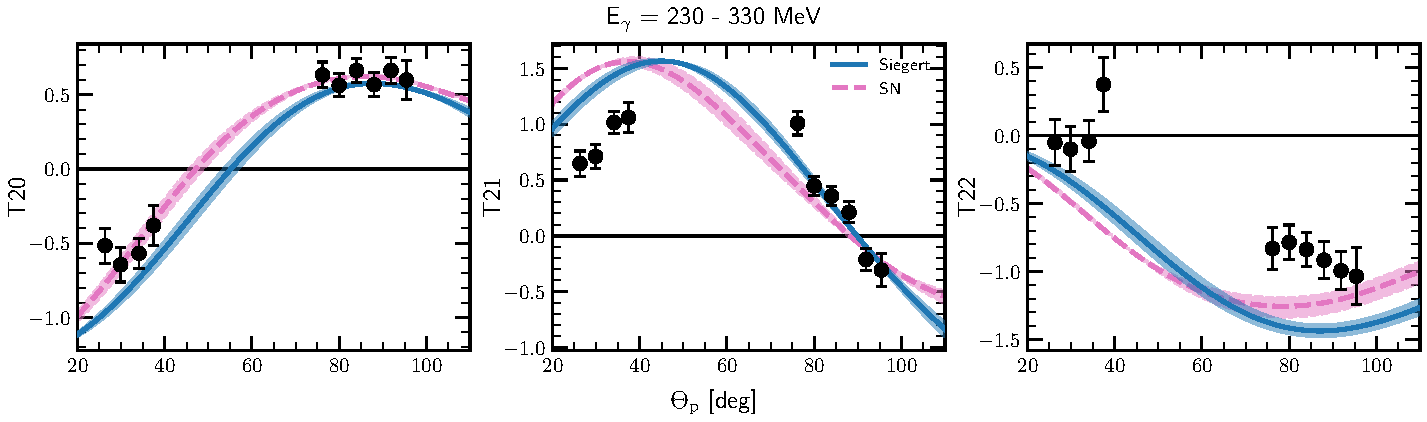
\includegraphics[width=0.95\textwidth]{Figures_De/Tensor_analyzing_power_angular_E230-330.pdf}
        \end{center}
        \caption{The same as on the Fig.~\ref*{tensor_angular_25-45} but for energy bin \SIrange{230}{330}{\mev}}
        \label{tensor_angular_230-330}
    \end{figure}
        


    On the Figure \ref{T20_vs_en} the energy dependance of $T_{20}$ and $T_{22}$
    (integrated over all angles)
    is presented for the energy range 0-400~MeV. I also demonstrate the experimental data from
    \cite{rachek2007} and \cite{mishev1993} as well as theoretical calculations from \cite{Schmitt1989}
    on the figure. For $T_{20}$ the model is able to describe experimental data well even for
    high energies. On the other hand, $T_{22}$ is not so well described: for the low 
    energies the prediction curve is somehow within uncertainties of experimental data,
    but further the difference with the data becomes larger. Also it is not 
    reflect the qualitative nature of the data as we can see that after around 150~MeV
    data points start ascending which is not represented in my predictions.
    Theoretical predictions from \cite{Schmitt1989} (brown dashed curve) are also not able
    to describe data quantitatively for $T_{22}$, but the growth is presented there. 

    Similar situation is on the Figures \ref{tensor_energy_24-48} and \ref{tensor_energy_70-102}
    where I show an energy dependance of Deuteron analyzing power components for 
    specific angular ranges (following the data from \cite{rachek2007}).
    Predictions for $T_{20}$ are able to reflect the experimental results,
    while for $T_{21}$ and $T_{22}$ predictions are reasonable (quantitative-wise) 
    only for lower energies and difference with data becomes larger
    when energy increases. Predictions for $T_{22}$ once more 
    confirm an insufficiency of SN and an importance of
    2-nucleon current contributions. 
    

    \begin{figure}[h]
        \begin{center}
        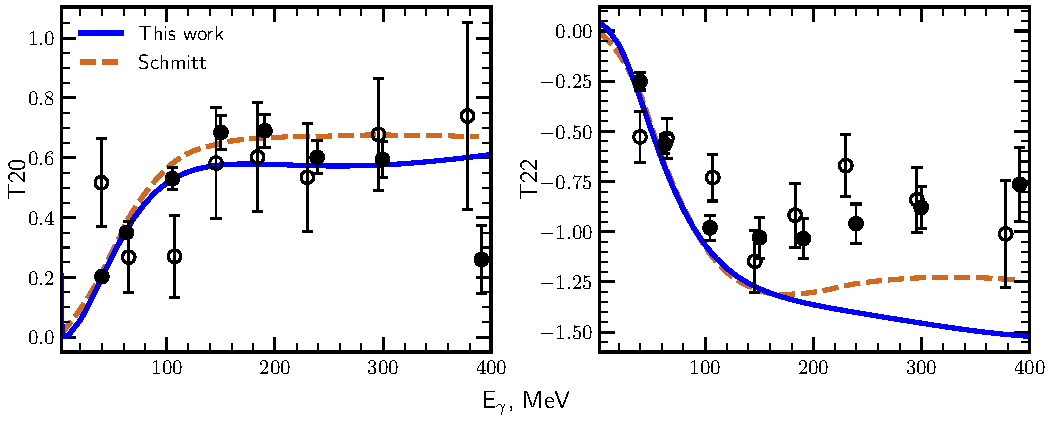
\includegraphics[width=0.9\textwidth]{Figures_De/T20_T22_vs_en.pdf}
        \end{center}
        \caption{Tensor analyzing powers T$_{20}$ and T$_{22}$ as a functions of the photon energy E$_\gamma$
        with fixed outgoing proton angle $\theta_p = 88^{\circ}$ (in the center of mass frame).
        My predictions (blue solid line) are obtained with \gls*{sms} potential at chiral order N$^4$LO+
        and with cutoff parameter $\Lambda$~=~450~MeV.
        Dashed brown line presents calculations from \cite{Schmitt1989}.
        Experimental data is taken from \cite{rachek2007} (filled circles)
        and \cite{mishev1993} (empty circles).}
        \label{T20_vs_en}
    \end{figure}

    \begin{figure}[h]
        \begin{center}
        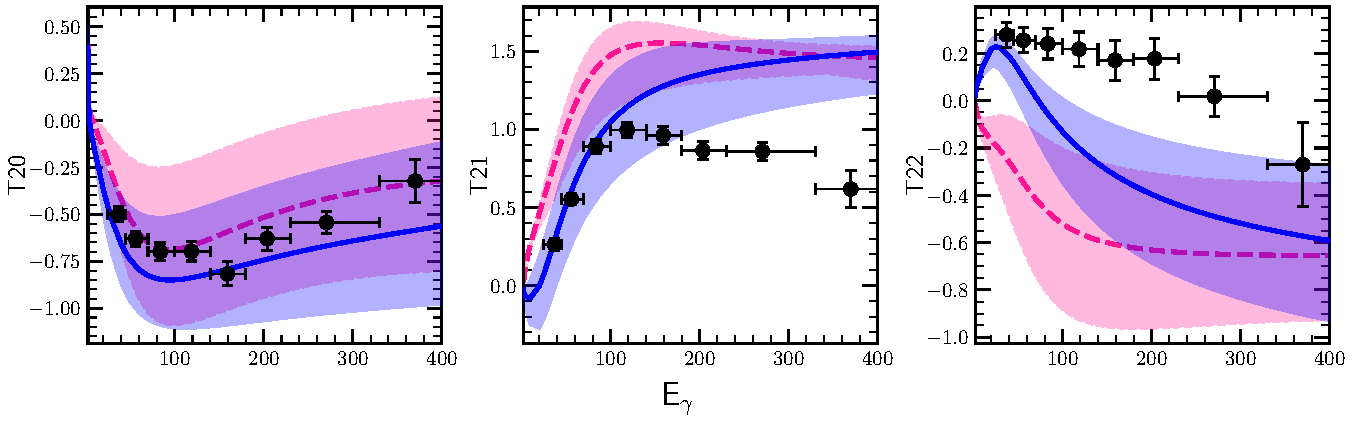
\includegraphics[width=0.95\textwidth]{Figures_De/TensorPower_Th24-48.pdf}
        \end{center}
        \caption{Tensor analyzing powers T$_{20}$, T$_{21}$ and T$_{22}$ as a functions of the
        photon's energy within the outgoing proton's angle range $24^{\circ} - 48^{\circ}$
        (in the center of mass frame).
        Solid blue line is a mean value of my predictions obtained with
        \gls*{sms} potential at N$^4$LO+ chiral order and with $\Lambda$~=~450~MeV
        at energy values from 25 to 45 MeV within
        a given angles range and
        where SN current was used together with Siegert approach. 
        Pink dashed line is similar prediction but with SN only. 
        The corresponding bands show the deviation of predictions in the regarded
        energy region.
        Filled circles are experimental data
        from \cite{rachek2007} for the analogous energy span.}
        \label{tensor_energy_24-48}
    \end{figure}

    \begin{figure}[h]
        \begin{center}
        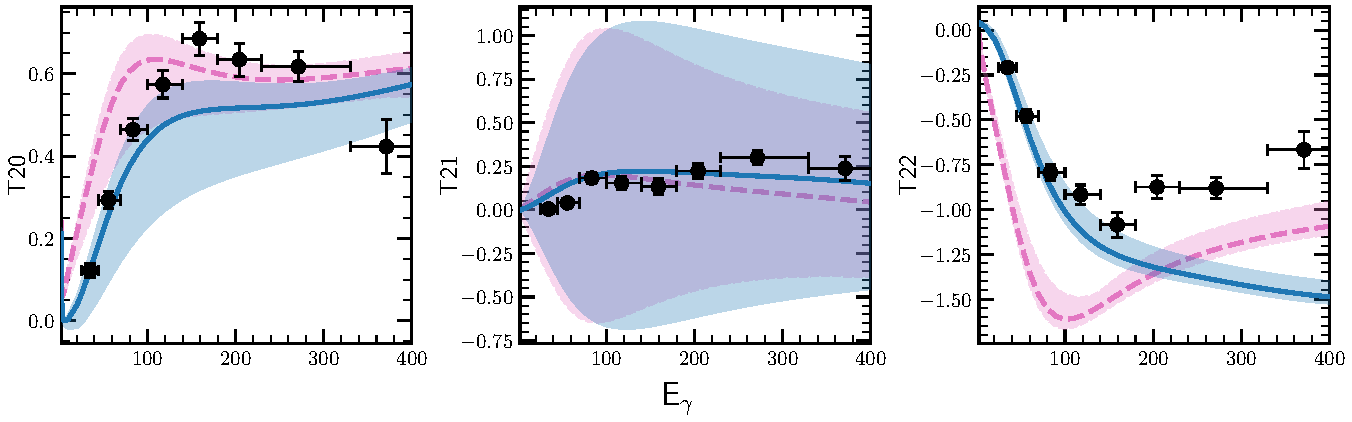
\includegraphics[width=0.95\textwidth]{Figures_De/TensorPower_Th70-102.pdf}
        \end{center}
        \caption{The same as on the Fig.~\ref*{tensor_energy_24-48} but
        for the angles' range $70^{\circ} - 102^{\circ}$.}
        \label{tensor_energy_70-102}
    \end{figure}
    
    On the \fig{assymetry} I demonstrate predictions
    for the photon asymmetry $\Sigma_\gamma$ for the 
    deuteron photodisintegraion with $E_\gamma$~=~20~MeV (a)
    and 60~MeV(b) as well as experimental data.
    Both (a) and (b) figureas are organized similarly to the 
    figures I showed earlier for the tensor analyzing power (e.g. \fig{T22_T11_30}).
    That is the top pane is aimed to demonstrate predictions obtained
    with chiral potential at different orders, the middle 
    one is showing a truncation error bands and the bottom - shows 
    the cutoff dependance. What we can see here is good 
    convergence with respect to the chiral order. For both regarded 
    energies predictions at different orders are very close to each other
    except for LO and NLO curves. Nevertheless, at 60~MeV we can see 
    that truncation error bands reveal some uncertainty connected 
    with the chiral order and I can assume that even some higher chiral 
    orders would still contribute to the predictions at this energy.

    Cutoff dependance is also stronger at 60~MeV. We can clearly see
    that predictions are different for each value of the $\Lambda$.
    The standard deviation with respect to the cutoff parameter at 20~MeV
    does not exceed 0.7\% of the mean value while at the photon's energy 60~MeV
     the maximum value is around 2.5\% (at $\theta = 115^\circ$).

     Regarding the correspondace to experimental data, we can clearly see that
     for the lower energy predictions are almost perfectly overlaping
     with exparimental point (and error bars). Few points are laying
     outside the predictions but it can be caused by experimental issues.
     For 60~MeV, experimental data points are constantly below prediction
     curves (especially in the middle of angles range). It seems that some systematic 
     uncertainty is presented in predictions and multiplication by some factor
     (presumably less than 1)
     could help predictions be more similar to experimental data.

     On the \fig{asymmetry_90deg} I present dependance of the asymmetry
     $\Sigma_\gamma$ on the photon's energy with fixed value
     of the outgoing proton's angle $\theta_p = 90^\circ$ 
     (following the data given at \cite{delbianco_1981} and \cite{depascale_asymmetry}).
     It is noticeable that with increasing energy, the prediction curve
     becomes more and more above the experimental data. This trend
     was also observed in angular dependance of the asymmetry at 60~MeV
     so I can assume that within our framework, 
     $\Sigma_\gamma$ is sensitive to the initial photon's energy and some 
     contributions are missing in order to prepare good predictions
     at higher energies. From the \fig{asymmetry_90deg} we can say that
     large descripancy with data starts appearing after 
     35~MeV. 

    % \begin{figure}[h]
    %     \centering
    %     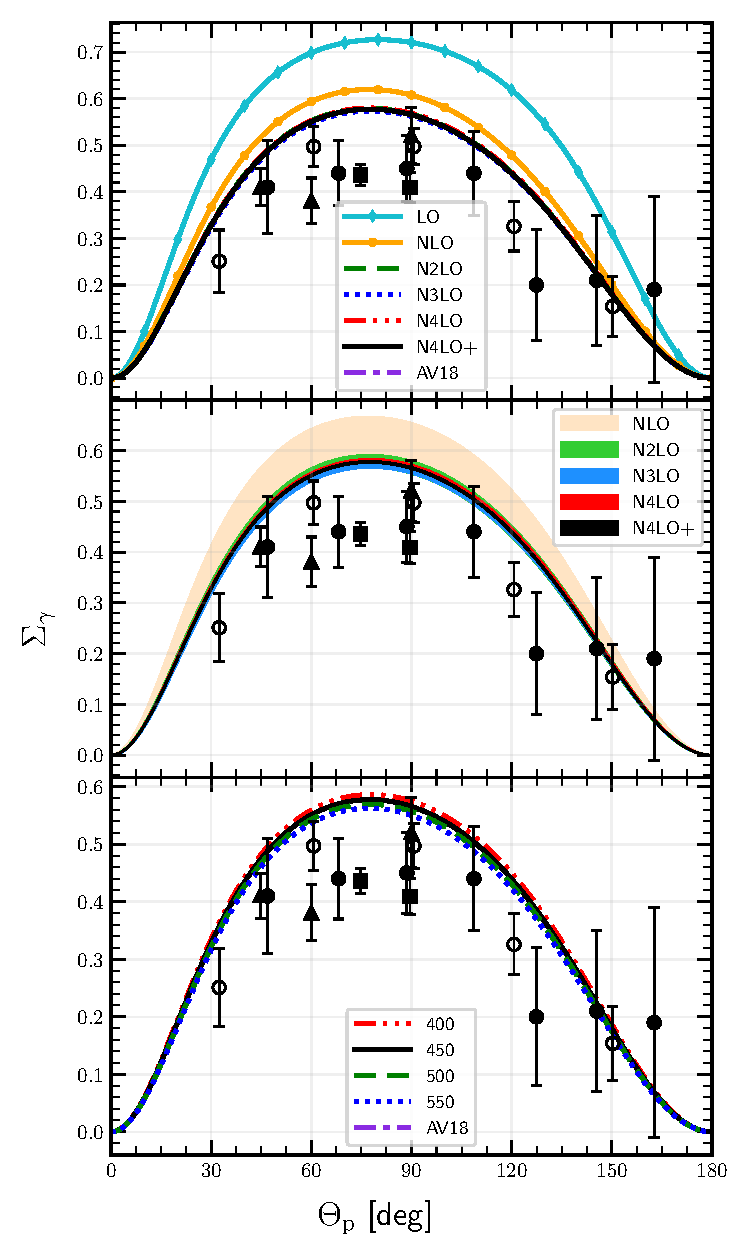
\includegraphics[width=0.65\textwidth]{Figures_De/AX2_60mev.pdf}
    %     % \caption{\small E$_\gamma = 30$~MeV}
    %     \caption{The photon asymmetry $\Sigma_\gamma$ 
    %     as a function of the outgoing proton angle in the center of mass frame 
    %     for the photon's energy 60 MeV.
    %     Top figure presents results obtained using potential
    %     with different chiral orders (from LO to N$^4$LO+) with cutoff parameter $\Lambda=450$~MeV.
    %     The middle pane shows truncation errors for each 
    %     chiral order starting from NLO and
    %     bottom figure presents a cutoff dependency (chiral potential N$^4$LO+).
    %     Filled circles are experimental data from \cite{KRAUSE1992_asymetry},
    %     empty circles - from \cite{depascale_asymmetry}, filled squares
    %     - from \cite{Barannik_asymetry} and triangles are from \cite{Vnukov_asymmetry}.
    %     For the sake of comparison, predictions obtained with \gls*{av18} potential are on  figures as well.}
    %     \label{assymetry_60mev}
    % \end{figure}

    \begin{figure}[h]
        \centering
        \begin{subfigure}[b]{0.46\textwidth}
            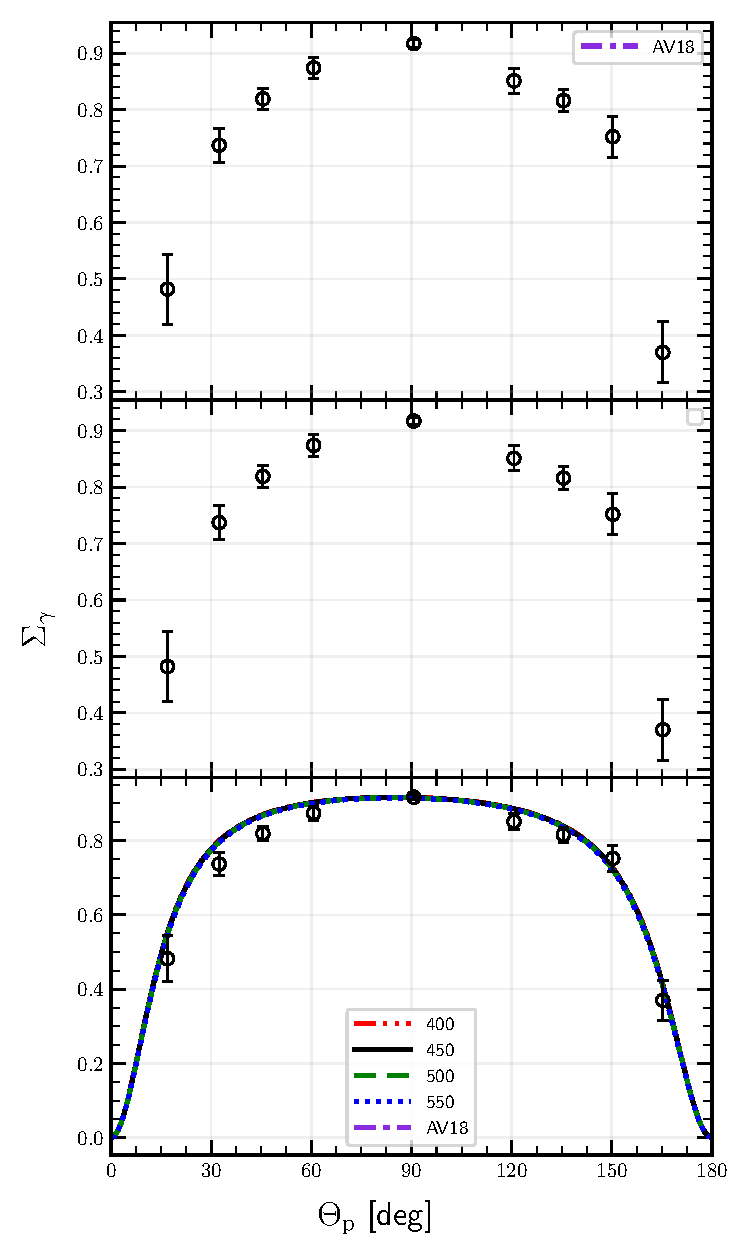
\includegraphics[width=\textwidth]{Figures_De/AX2_20mev.pdf}
            \caption{\small E$_\gamma = 20$~MeV}
            \label{AX_20_vert}
        \end{subfigure}
        \begin{subfigure}[b]{0.46\textwidth}
            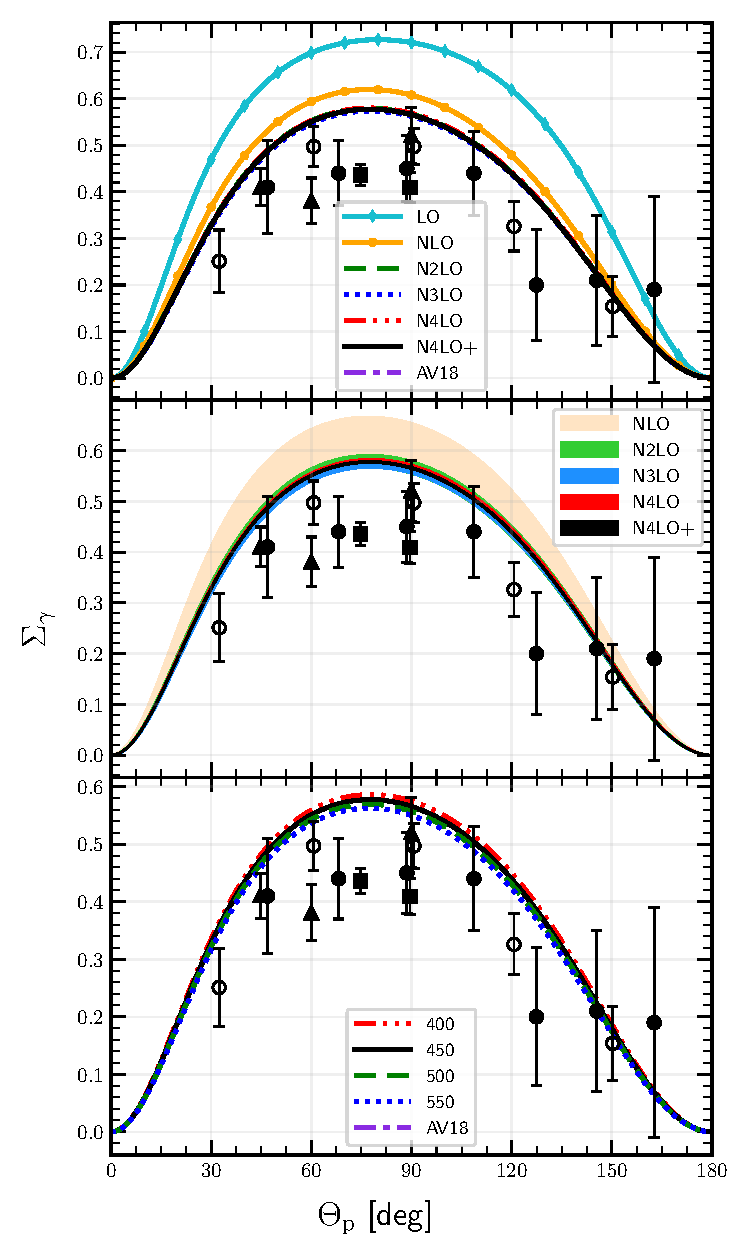
\includegraphics[width=\textwidth]{Figures_De/AX2_60mev.pdf}
            \caption{\small E$_\gamma = 60$~MeV}
            \label{AX_60_vert}
        \end{subfigure}
        \caption{The photon asymmetry $\Sigma_\gamma$ 
        as a function of the outgoing proton angle in the center of mass frame 
        for the photon's energy \SI{30}{\mev}(a) and \SI{100}{\mev}(b).
        Top row presents results obtained using potential
        with different chiral orders (from LO to N$^4$LO+) with cutoff parameter $\Lambda=450$~MeV.
        The middle row shows truncation errors for each 
        chiral order starting from NLO and
        bottom presents a cutoff dependency (chiral potential N$^4$LO+).
        Filled circles are experimental data from \cite{KRAUSE1992_asymetry},
        empty circles - from \cite{depascale_asymmetry}, filled squares
        - from \cite{Barannik_asymetry} and triangles are from \cite{Vnukov_asymmetry}.
        For the sake of comparison, predictions obtained with \gls*{av18} potential are on  figures as well.}
        \label{assymetry}
    \end{figure}
     
    \begin{figure}[h]
        \begin{center}
        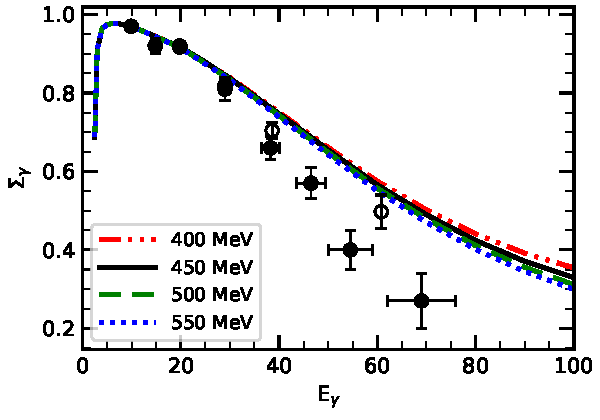
\includegraphics[width=0.75\textwidth]{Figures_De/AX2_90deg.pdf}
        \end{center}
        \caption{The photon asymmetry $\Sigma_\gamma$ 
        as a function of the photon energy  
        with fixed outgoing proton angle $\theta_p=90^\circ$.
        Each curve corresponds to the particular value of the cutoff parameter
        and chiral potential used here is N$^4$LO+.
        Filled circles are experimental data from \cite{delbianco_1981},
        empty circles - from \cite{depascale_asymmetry}.}
        \label{asymmetry_90deg}
    \end{figure}
    

    The proton polarization is demonstrated on the \fig{PY_30_100_vert} for the 
    photon's energy 30~MeV(a) and 100~MeV(b). In this case even higher energy
    such as 100~MeV does not reveal neither
    slower convergence with respect to the chiral order no
    stronger cutoff dependence. Figures for both energies show
    that only next-to-leading order brings relatively high contribution
    while taking into account each subsequent order does not change predictions
    largely. In the case of cutoff dependance, we see that curves for each
    value of $\Lambda$ are very close to each other. 
    The standard deviation of the predictions with respect to the cutoff parameter
    has maximal value 1.94\% at $E_\gamma = 30$MeV and 3.2\% at 100~MeV.
    The dependance is slightly stronger for higher energy, but these values are comparable.


    \begin{figure}[h]
        \centering
        \begin{subfigure}[b]{0.46\textwidth}
            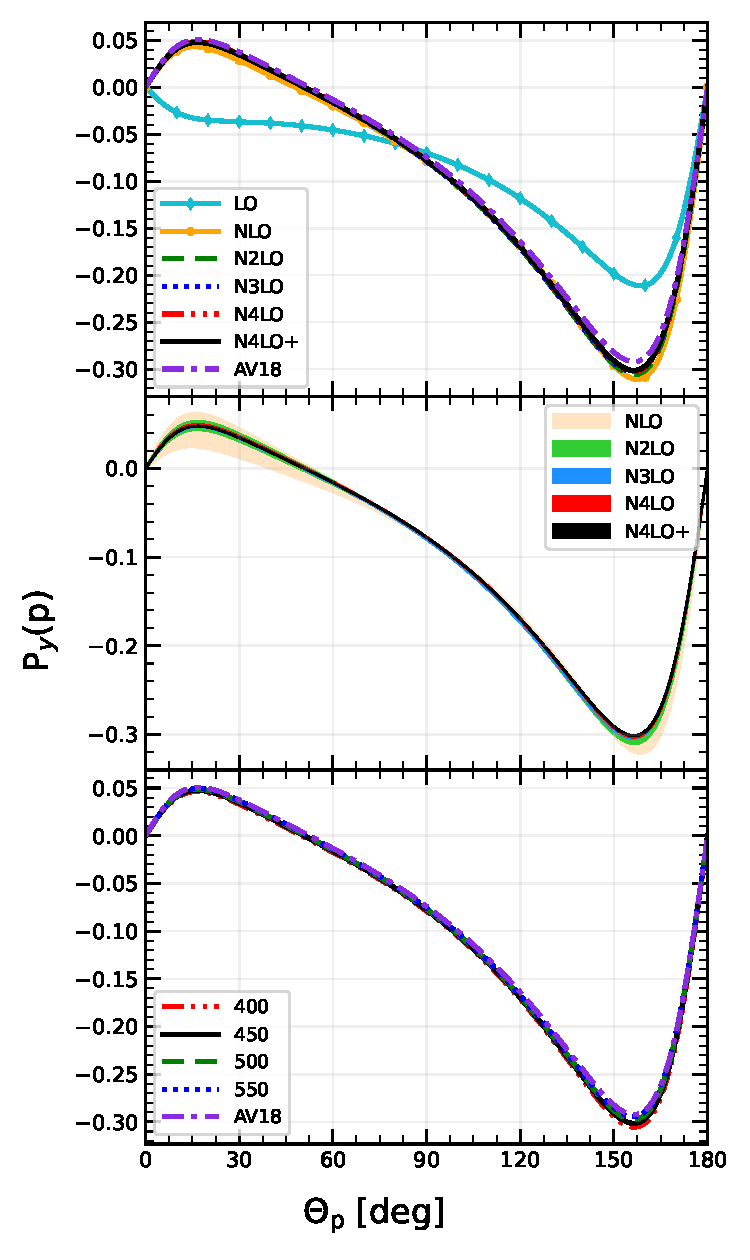
\includegraphics[width=\textwidth]{Figures_De/POLNOUT2(y)_30mev.pdf}
            \caption{\small E$_\gamma = 30$~MeV}
            \label{PY_30_vert}
        \end{subfigure}
        \begin{subfigure}[b]{0.46\textwidth}
            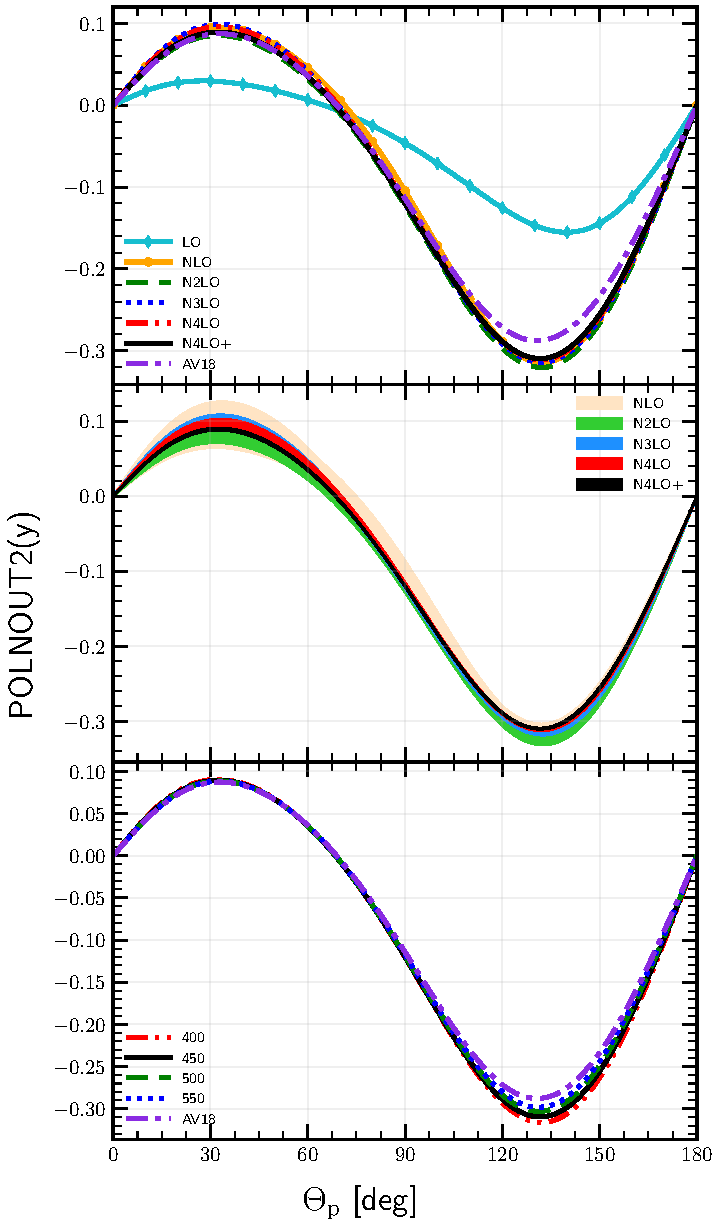
\includegraphics[width=\textwidth]{Figures_De/POLNOUT2(y)_100mev.pdf}
            \caption{\small E$_\gamma = 100$~MeV}
            \label{PY_100_vert}
        \end{subfigure}
        \caption{Proton polarisation $P_y(p)$ 
        \label{PY_30_100_vert}
        as a function of the outgoing proton angle in the center of mass frame 
        for the photon's energy \SI{30}{\mev} (a) and \SI{100}{\mev} (b).
        Top figure presents results obtained using potential
        with different chiral orders (from LO to N$^4$LO+) with cutoff parameter $\Lambda=450$~MeV.
        The middle pane shows truncation errors for each 
        chiral order starting from NLO and
        bottom figure presents a cutoff dependency (chiral potential N$^4$LO+).
        For the sake of comparison, predictions obtained with \gls*{av18} potential are on  figures as well.}
    \end{figure}


    Predictions for the neuteron polarization at energy 2.75~MeV are on the
    \fig{Pn_2p75_vert}. The choice of energy is conditioned by the availability of experimental data.
    We can see that predictions reflect the behavior of experimental data points qualitatively,
    having more o less constant offset of the values. Similar offset was obtained
    also in predictions at \cite{ArenhovelPhotodisint1991}, where various approaches were presented.
    Interesting is that predictions clearly show symmetrical form of the curve, while in the experimental data
    have some deviations from symmetrical form. It can be a sign that some problem with data can be
    in this case (taking into account also that experiment had been done in 196) as well 
    as inaccuracy in theoretical models.

    \begin{figure}[h]
        % \centering
        % 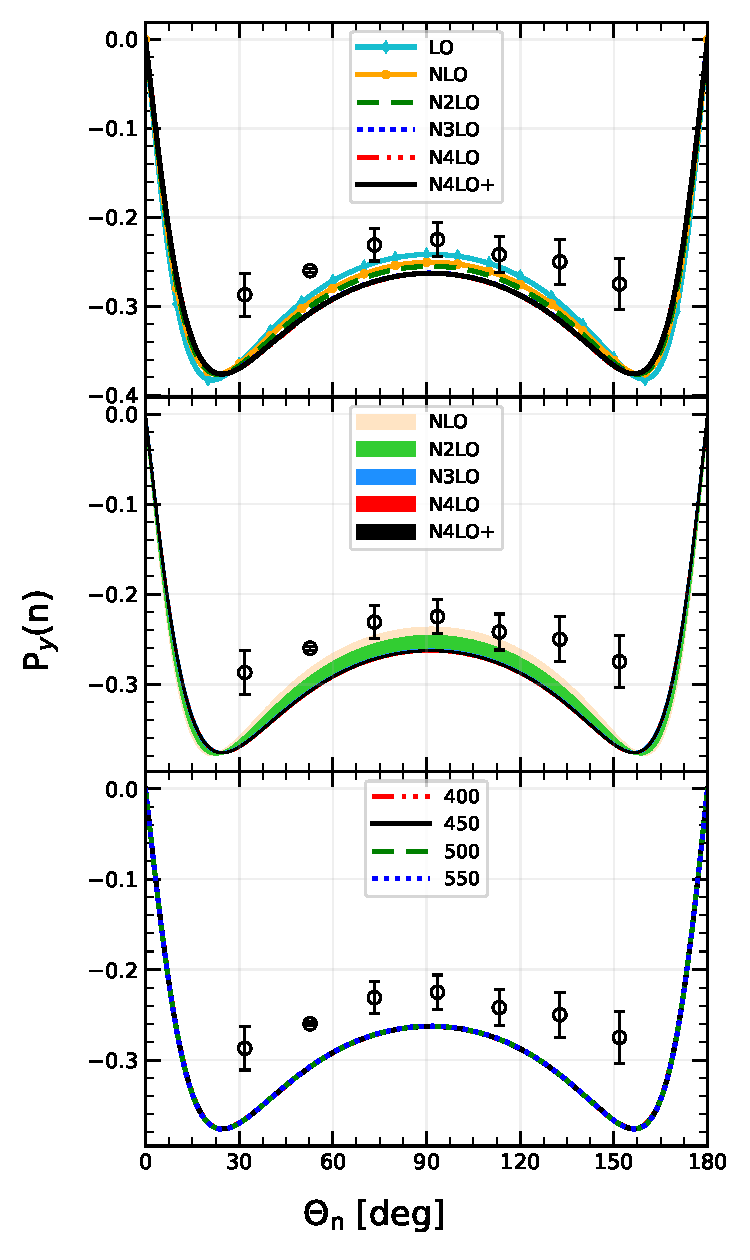
\includegraphics[width=0.5\textwidth]{Figures_De/POLNOUT2(y)_2.75mev_neuteron.pdf}
        \centering
        \begin{subfigure}[b]{0.46\textwidth}
            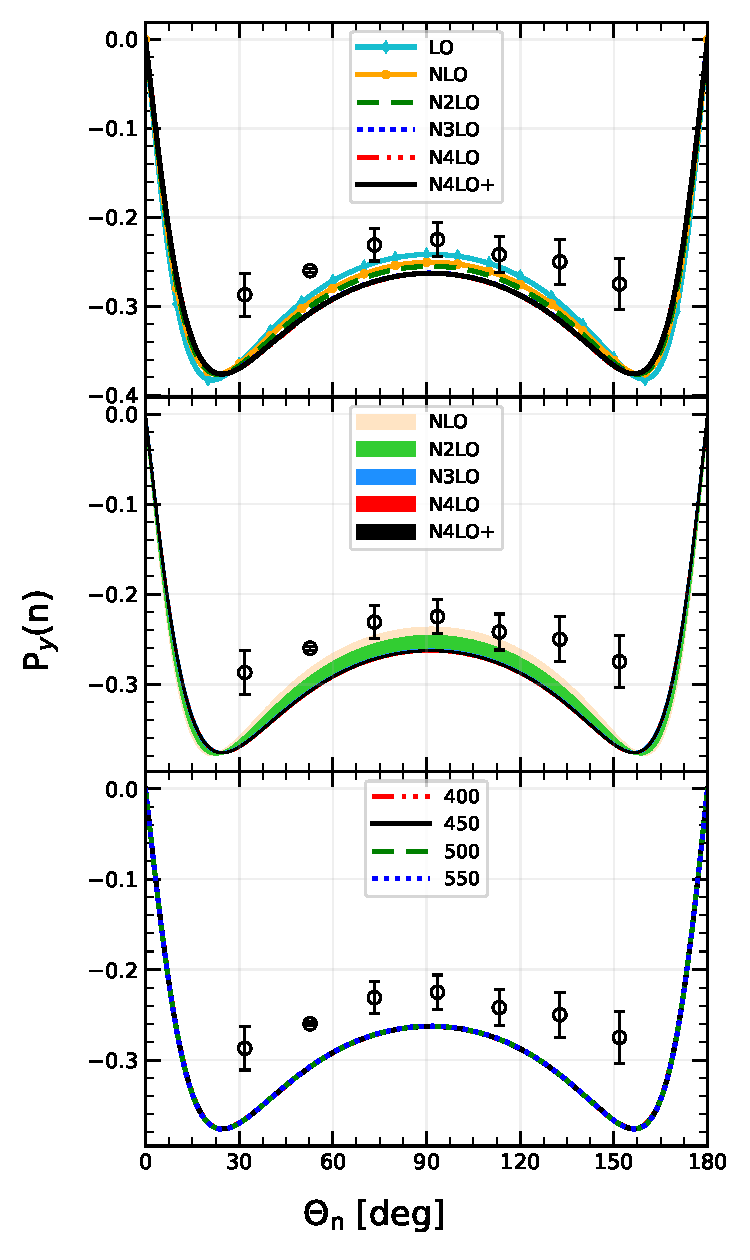
\includegraphics[width=\textwidth]{Figures_De/POLNOUT2(y)_2.75mev_neuteron.pdf}
            \caption{\small E$_\gamma = 2.75$~MeV}
            \label{Pn_30_vert}
        \end{subfigure}
        \begin{subfigure}[b]{0.46\textwidth}
            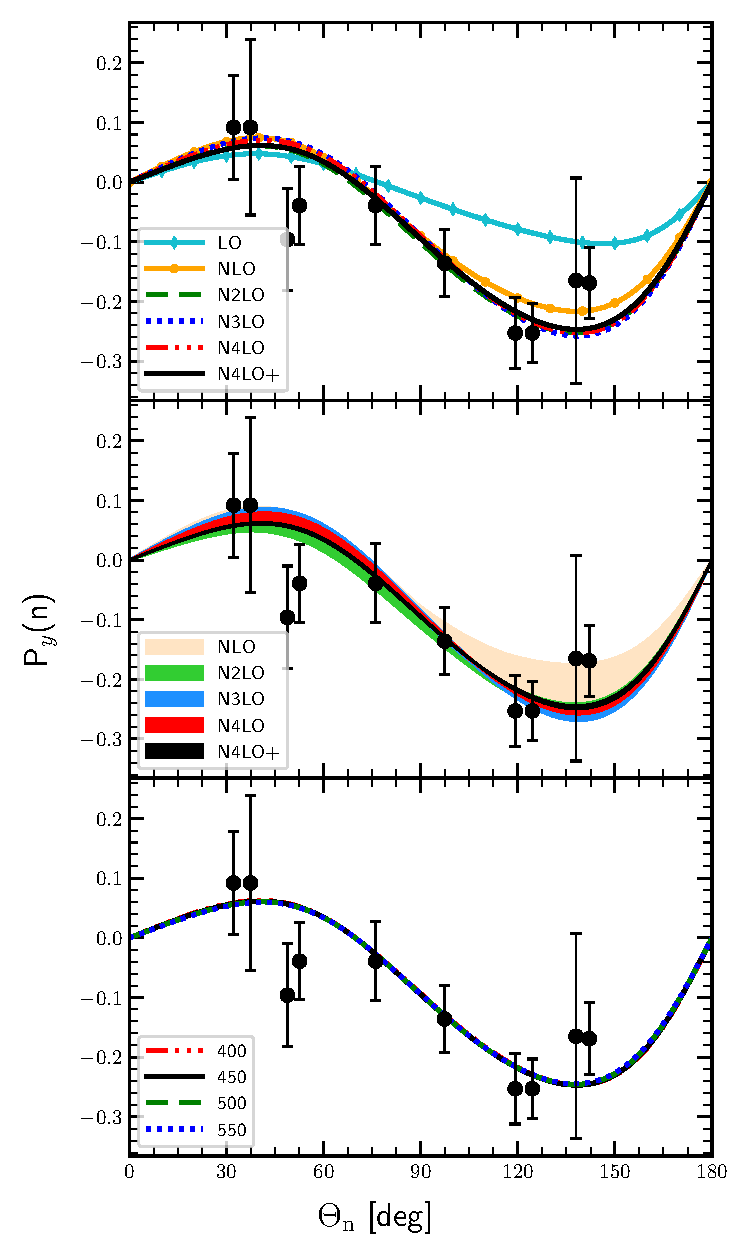
\includegraphics[width=\textwidth]{Figures_De/POLNOUT2(y)_100mev_neuteron.pdf}
            \caption{\small E$_\gamma = 100$~MeV}
            \label{Pn_100_vert}
        \end{subfigure}
        \caption{Neuteron polarisation $P_y(n)$ 
        as a function of the outgoing neuteron angle in the center of mass frame 
        for the photon's energy 2.75 MeV(a) and 100~MeV(b).
        Top row presents results obtained using potential
        with different chiral orders (from LO to N$^4$LO+) with cutoff parameter $\Lambda=450$~MeV.
        The middle pane shows truncation errors for each 
        chiral order starting from NLO and
        bottom figure presents a cutoff dependency (chiral potential N$^4$LO+).
        Experimental data is from \cite{Jewell_neuteronpolarization} (empty circles)
        and \cite{CAMERON_neuteronpolarization} (filled circles).}
        \label{Pn_2p75_100}
    \end{figure}


\clearpage

\section{Helium photodisintegration}

\subsection{3N photodisintegration}
    \begin{figure}[h]
        \begin{center}
            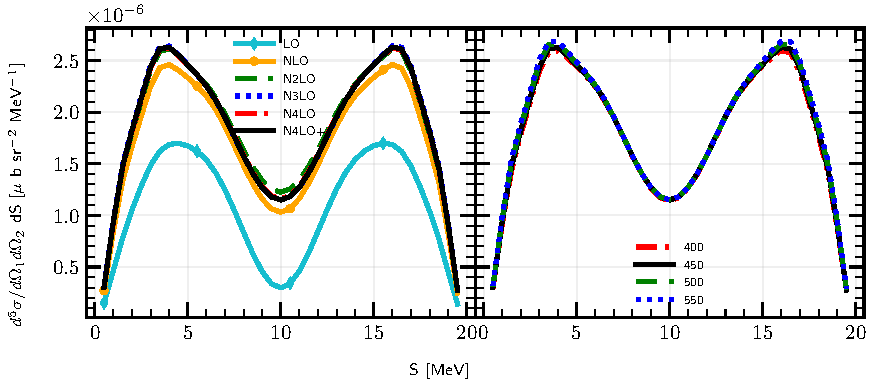
\includegraphics[width=0.9\textwidth]{Figures_HE/CROSS_excl_30mev.pdf}
            \end{center}
            \caption{The five-fold differential cross section for the photon 
            energy E$_\gamma=30$~MeV for the kinematic configuration
            $\theta_1 = 15^\circ$, $\phi_1 = 0^\circ$,
            $\theta_2 = 15^\circ$, $\phi_2 = 180^\circ$.
            The left figure presents results obtained using potential
            with different chiral orders (from LO to N$^4$LO+) with cutoff parameter $\Lambda=450$~MeV.
            The right figure presents a cutoff dependency (chiral potential N$^4$LO+).}
            \label{CROSS_HE_EXCL_30}
        \end{figure}


        \begin{figure}[h]
            \begin{center}
            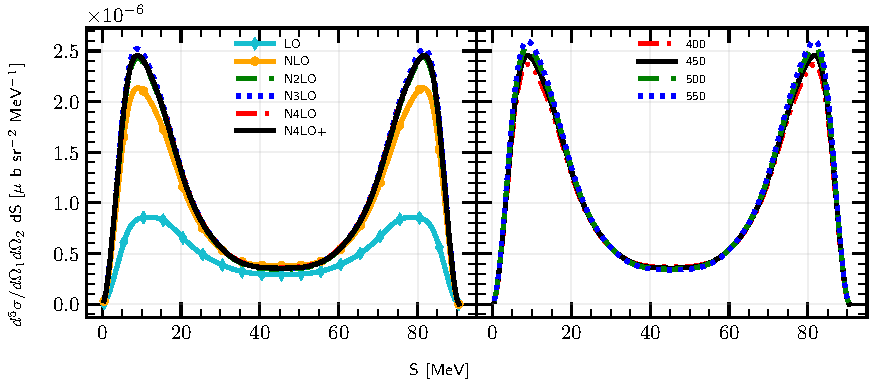
\includegraphics[width=0.9\textwidth]{Figures_HE/CROSS_excl_100mev.pdf}
            \end{center}
            \caption{The same as on Fig.~\ref{CROSS_HE_EXCL_30} but 
            for the photon energy E$_\gamma=100$~MeV}
            \label{CROSS_HE_EXCL_100}
        \end{figure}

        \begin{figure}[h]
            \begin{center}
                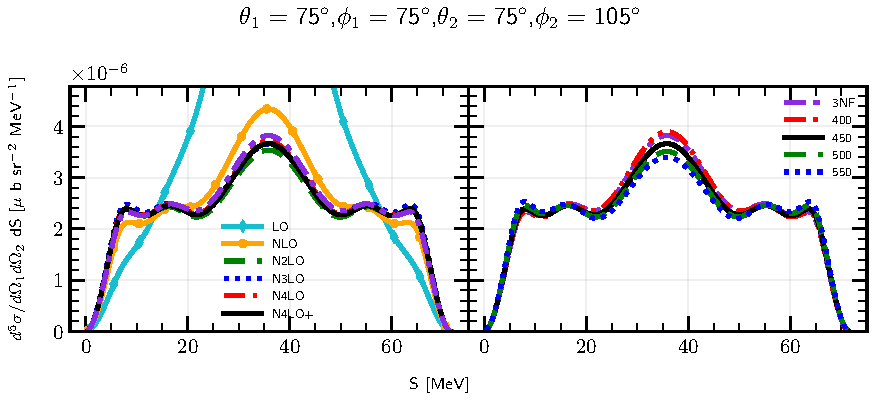
\includegraphics[width=0.9\textwidth]{Figures_HE/CROSS_excl_100mev_75_75_75_105.pdf}
                \end{center}
                \caption{The five-fold differential cross section for the photon 
                energy E$_\gamma=100$~MeV.
                The left figure presents results obtained using potential
                with different chiral orders (from LO to N$^4$LO+) with cutoff parameter $\Lambda=450$~MeV.
                The right figure presents a cutoff dependency (chiral potential N$^4$LO+).}
                \label{CROSS_HE_EXCL_75_75_75_105}
        \end{figure}

        \begin{figure}[h]
            \begin{center}
                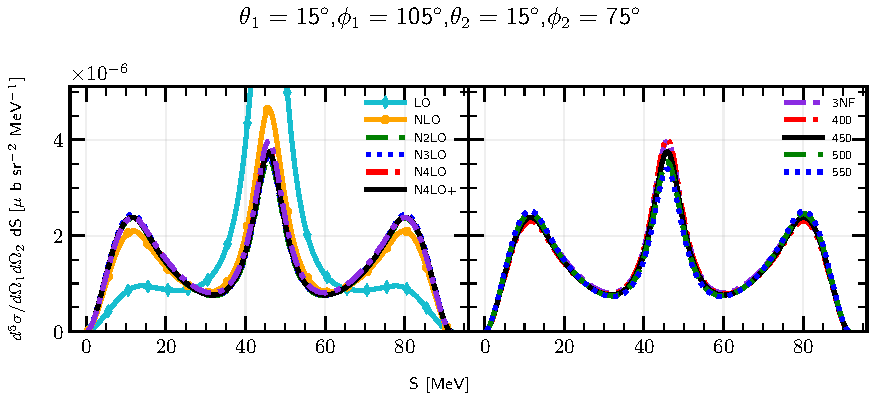
\includegraphics[width=0.9\textwidth]{Figures_HE/CROSS_excl_100mev_15_105_15_75.pdf}
                \end{center}
                \caption{The five-fold differential cross section for the photon 
                energy E$_\gamma=100$~MeV.
                The left figure presents results obtained using potential
                with different chiral orders (from LO to N$^4$LO+) with cutoff parameter $\Lambda=450$~MeV.
                The right figure presents a cutoff dependency (chiral potential N$^4$LO+).}
                \label{CROSS_HE_EXCL_15_105_15_75}
        \end{figure}

        \begin{figure}[h]
            \begin{center}
                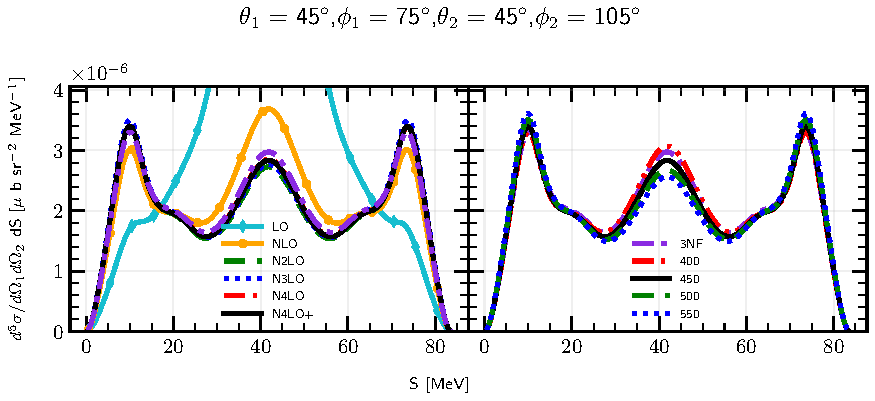
\includegraphics[width=0.9\textwidth]{Figures_HE/CROSS_excl_100mev_45_75_45_105.pdf}
                \end{center}
                \caption{The five-fold differential cross section for the photon 
                energy E$_\gamma=100$~MeV.
                The left figure presents results obtained using potential
                with different chiral orders (from LO to N$^4$LO+) with cutoff parameter $\Lambda=450$~MeV.
                The right figure presents a cutoff dependency (chiral potential N$^4$LO+).}
                \label{CROSS_HE_EXCL_45_75_45_105}
        \end{figure}

        \begin{figure}[h]
            \begin{center}
                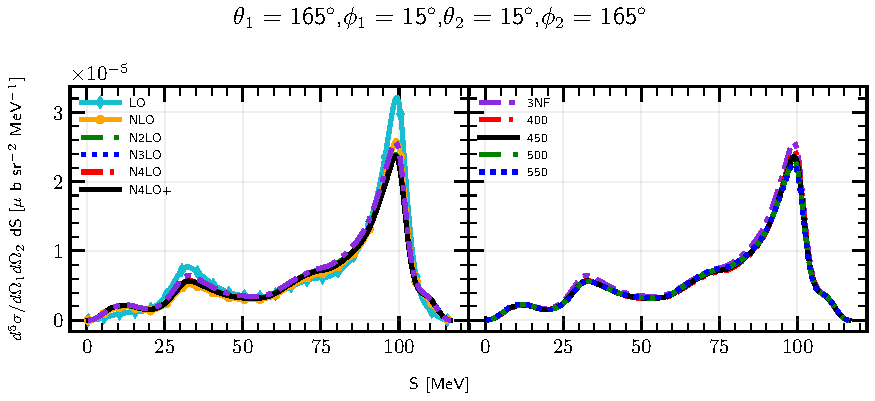
\includegraphics[width=0.9\textwidth]{Figures_HE/CROSS_excl_100mev_165_15_15_165.pdf}
                \end{center}
                \caption{The five-fold differential cross section for the photon 
                energy E$_\gamma=100$~MeV.
                The left figure presents results obtained using potential
                with different chiral orders (from LO to N$^4$LO+) with cutoff parameter $\Lambda=450$~MeV.
                The right figure presents a cutoff dependency (chiral potential N$^4$LO+).}
                \label{CROSS_HE_EXCL_165_15_15_165}
        \end{figure}



        \begin{figure}[h]
            \begin{center}
            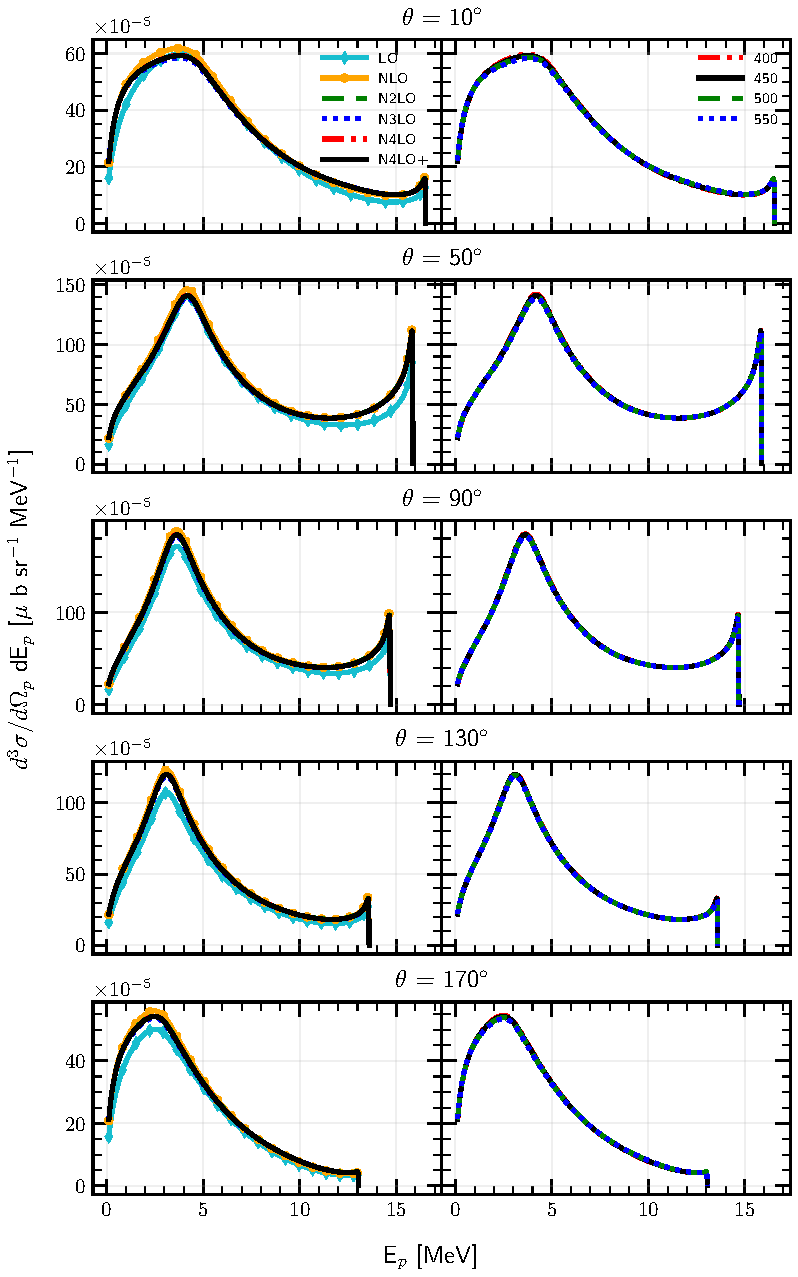
\includegraphics[width=0.9\textwidth]{Figures_HE/CROSS_incl_30mev_all.pdf}
            \end{center}
            \caption{Inclusive cross section. E$_\gamma$=30~MeV}
        \end{figure}

        \begin{figure}[h]
            \begin{center}
            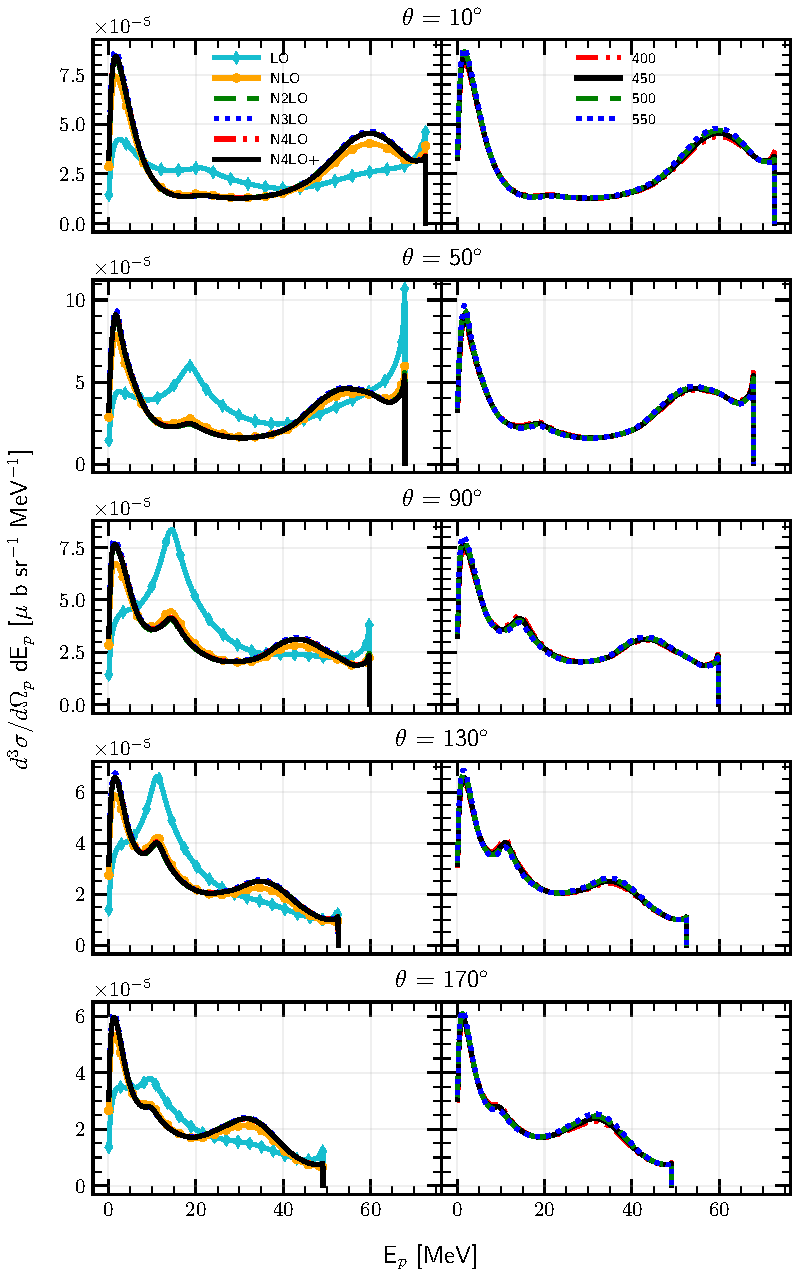
\includegraphics[width=0.9\textwidth]{Figures_HE/CROSS_incl_100mev_all.pdf}
            \end{center}
            \caption{Inclusive cross section. E$_\gamma$=100~MeV}
        \end{figure}


\clearpage


\subsection{Nd photodisintegration}

\begin{figure}[h]
    \begin{center}
        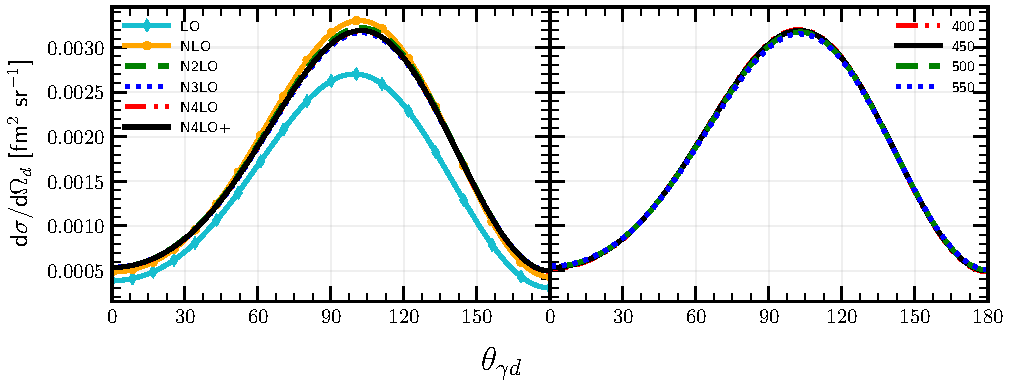
\includegraphics[width=0.9\textwidth]{Figures_HE/CROSS_nd_30mev.pdf}
        \end{center}
        \caption{Differential cross section for the d-$\gamma$ 
        two-body photodisintegraion of $^3$He as a function of the d$\gamma$ angle.
        The initial photon energy $E_\gamma=30$~MeV.}
        \label{CROSS_nd_30}
    \end{figure}


    \begin{figure}[h]
        \begin{center}
        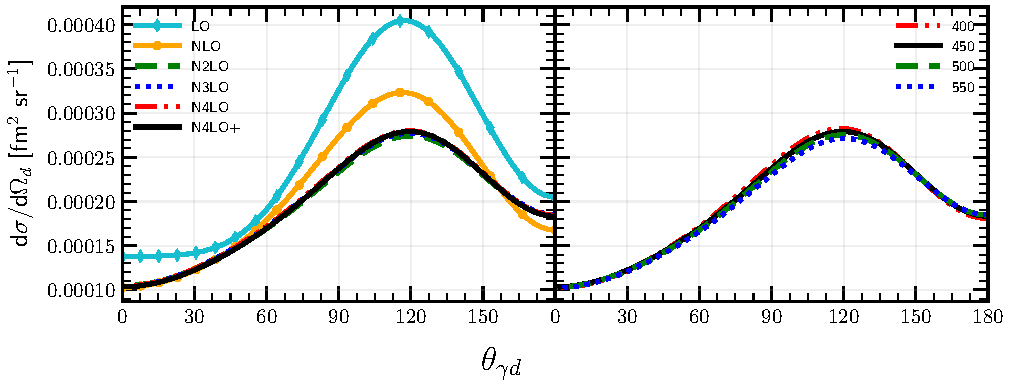
\includegraphics[width=0.9\textwidth]{Figures_HE/CROSS_nd_100mev.pdf}
        \end{center}
        \caption{The same as on Fig.~\ref{CROSS_nd_30} but 
        for the photon energy E$_\gamma=100$~MeV}
        \label{CROSS_nd_100}
    \end{figure}

    \clearpage
    \section{Pion absorption from the lowes atomic orbital}

    \subsection{Pion absorption in $^3$He}

    \begin{figure}[h]
        \begin{center}
        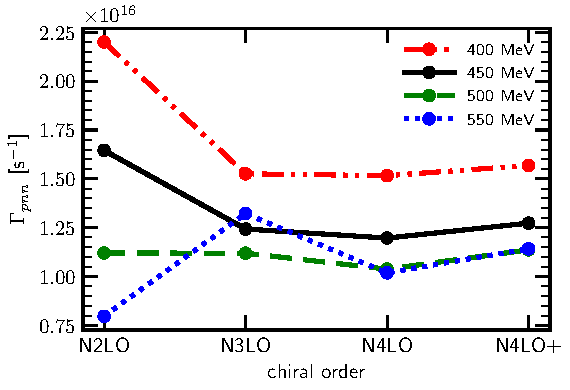
\includegraphics[width=0.6\textwidth]{PlotData/PION/Dalitz_maps/figures/Gamma_pnn.pdf}
        \end{center}
        \caption{}
        \label{Gamma_pnn}
    \end{figure}

    \begin{figure}[h]
        \begin{center}
        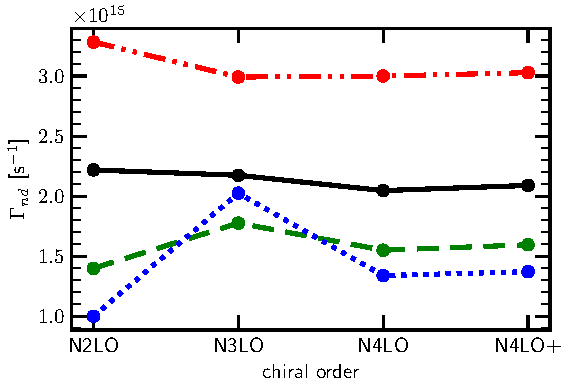
\includegraphics[width=0.6\textwidth]{PlotData/PION/Dalitz_maps/figures/Gamma_nd.pdf}
        \end{center}
        \caption{}
        \label{Gamma_nd}
    \end{figure}

    \begin{figure}[h]
        \begin{center}
        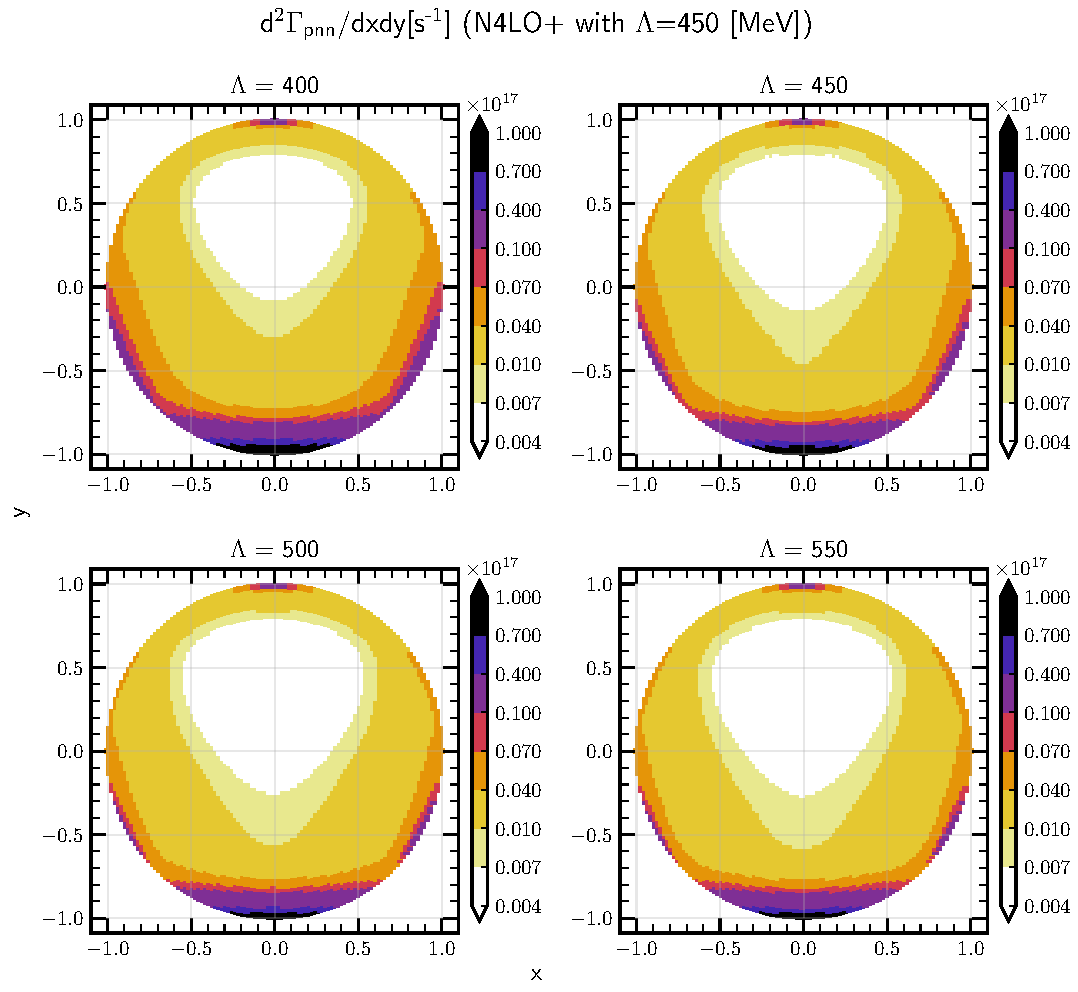
\includegraphics[width=0.7\textwidth]{PlotData/PION/Dalitz_maps/figures/Dalitz_map_pnn_xy_cutofs.pdf}
        \end{center}
        \caption{}
        \label{pion_map_xy_cutoff}
    \end{figure}

    \begin{figure}[h]
        \begin{center}
        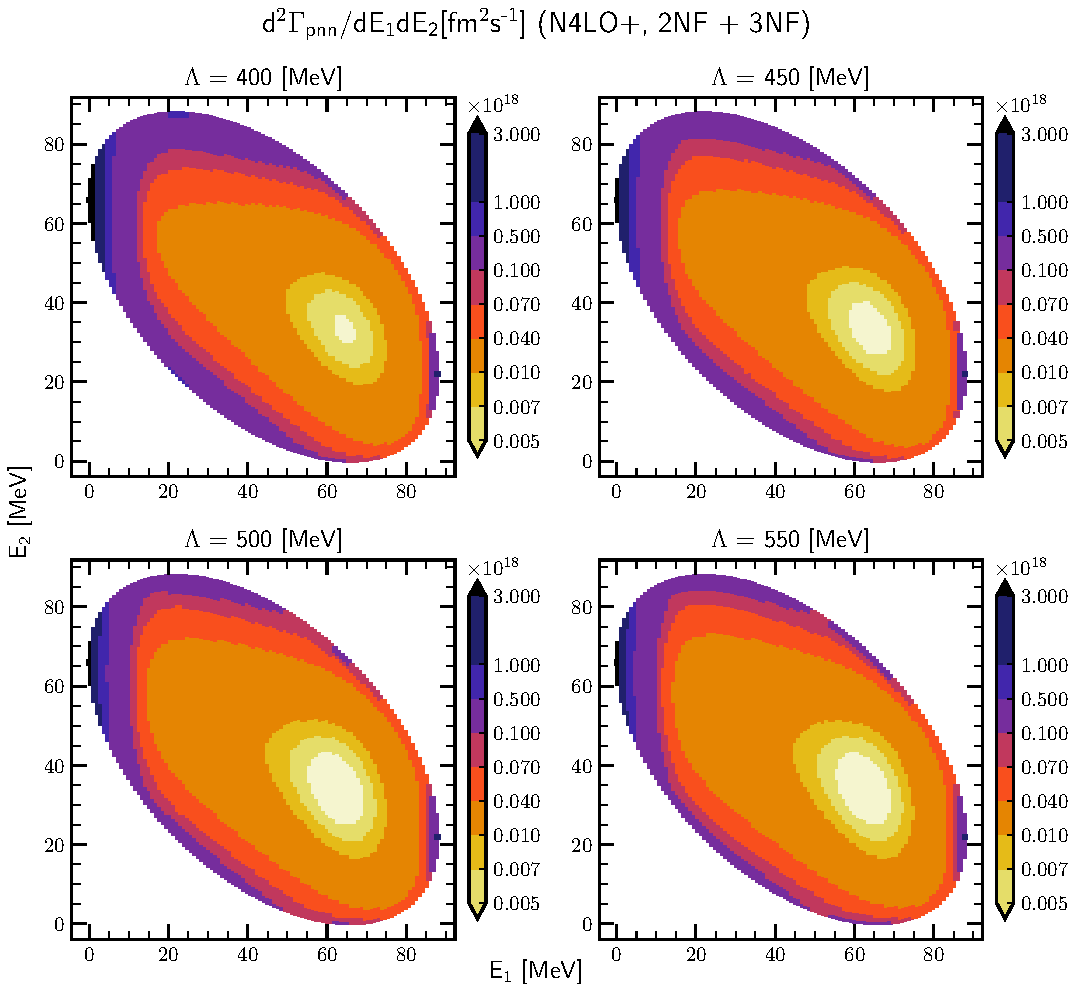
\includegraphics[width=0.7\textwidth]{PlotData/PION/Dalitz_maps/figures/Dalitz_map_pnn_E1E2_cutofs.pdf}
        \end{center}
        \caption{}
        \label{pion_map_E1E2_cutoff}
    \end{figure}

    \begin{figure}[h]
        \begin{center}
        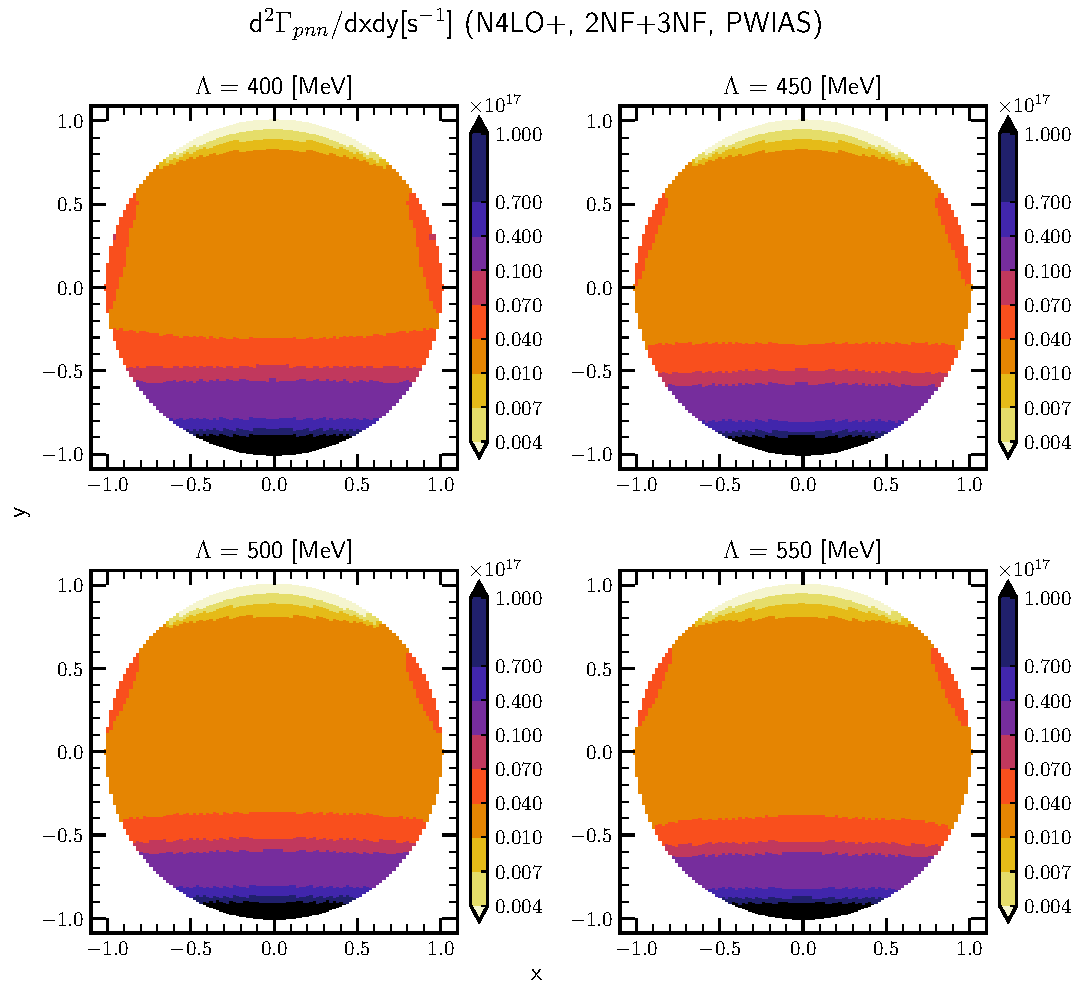
\includegraphics[width=0.7\textwidth]{PlotData/PION/Dalitz_maps/figures/Dalitz_map_pnn_xy_cutofs_PWIAS.pdf}
        \end{center}
        \caption{}
        \label{pion_map_xy_cutoff_PW}
    \end{figure}

    \begin{figure}[h]
        \begin{center}
        \includegraphics[width=0.7\textwidth]{PlotData/PION/Dalitz_maps/figures/Dalitz_map_pnn_E1E2_cutofs_PWIAS.pdf}
        \end{center}
        \caption{}
        \label{pion_map_E1E2_cutoff_PW}
    \end{figure}

    \begin{figure}[h]
        \begin{center}
        \includegraphics[width=0.7\textwidth]{PlotData/PION/Dalitz_maps/figures/Dalitz_map_pnn_xy_cutofs_1NC.pdf}
        \end{center}
        \caption{}
        \label{pion_map_xy_cutoff_1NC}
    \end{figure}

    \begin{figure}[h]
        \begin{center}
        \includegraphics[width=0.7\textwidth]{PlotData/PION/Dalitz_maps/figures/Dalitz_map_pnn_E1E2_cutofs_1NC.pdf}
        \end{center}
        \caption{}
        \label{pion_map_E1E2_cutoff_1NC}
    \end{figure}

    \begin{figure}[h]
        \begin{center}
        \includegraphics[width=0.7\textwidth]{PlotData/PION/Dalitz_maps/figures/Dalitz_map_pnn_xy_orders.pdf}
        \end{center}
        \caption{}
        \label{pion_map_xy_order}
    \end{figure}

    \begin{figure}[h]
        \begin{center}
        \includegraphics[width=0.7\textwidth]{PlotData/PION/Dalitz_maps/figures/Dalitz_map_pnn_E1E2_orders.pdf}
        \end{center}
        \caption{}
        \label{pion_map_E1E2_order}
    \end{figure}

    \begin{figure}[h]
        \begin{center}
        \includegraphics[width=0.9\textwidth]{PlotData/PION/Dalitz_maps/figures/3HE_dGdEp.pdf}
        \end{center}
        \caption{}
        \label{pion_GdEp}
    \end{figure}

    \begin{figure}[h]
        \begin{center}
        \includegraphics[width=0.9\textwidth]{PlotData/PION/Dalitz_maps/figures/3HE_dGdEn.pdf}
        \end{center}
        \caption{}
        \label{pion_dGdEn}
    \end{figure}

    \begin{figure}[h]
        \begin{center}
        \includegraphics[width=0.9\textwidth]{PlotData/PION/Dalitz_maps/figures/3HE_dGdr.pdf}
        \end{center}
        \caption{}
        \label{pion_dGdEr}
    \end{figure}

    \begin{figure}[h]
        \begin{center}
        \includegraphics[width=0.9\textwidth]{PlotData/PION/Dalitz_maps/figures/3HE_dGdphi.pdf}
        \end{center}
        \caption{}
        \label{pion_dGdphi}
    \end{figure}


    \clearpage
    \subsection{$\pi^- + ^3$H $\rightarrow n + n + n$}

    \begin{figure}[h]
        \begin{center}
        \includegraphics[width=0.6\textwidth]{PlotData/PION/Dalitz_maps/figures/Gamma_nnn.pdf}
        \end{center}
        \caption{}
        \label{Gamma_nnn}
    \end{figure}


    \begin{figure}[h]
        \begin{center}
        \includegraphics[width=0.7\textwidth]{PlotData/PION/Dalitz_maps/figures/Dalitz_map_nnn_xy_cutofs.pdf}
        \end{center}
        \caption{}
        \label{pion_nnn_xy_cutoff}
    \end{figure}

    \begin{figure}[h]
        \begin{center}
        \includegraphics[width=0.7\textwidth]{PlotData/PION/Dalitz_maps/figures/Dalitz_map_nnn_E1E2_cutofs.pdf}
        \end{center}
        \caption{}
        \label{pion_nnn_E1E2_cutoff}
    \end{figure}

    \begin{figure}[h]
        \begin{center}
        \includegraphics[width=0.7\textwidth]{PlotData/PION/Dalitz_maps/figures/Dalitz_map_nnn_xy_orders.pdf}
        \end{center}
        \caption{}
        \label{pion_nnn_xy_order}
    \end{figure}

    \begin{figure}[h]
        \begin{center}
        \includegraphics[width=0.7\textwidth]{PlotData/PION/Dalitz_maps/figures/Dalitz_map_nnn_E1E2_orders.pdf}
        \end{center}
        \caption{}
        \label{pion_nnn_E1E2_order}
    \end{figure}

    \begin{figure}[h]
        \begin{center}
        \includegraphics[width=0.9\textwidth]{PlotData/PION/Dalitz_maps/figures/3H_dGdEn.pdf}
        \end{center}
        \caption{}
        \label{pion_dGdEn_3H}
    \end{figure}

    \begin{figure}[h]
        \begin{center}
        \includegraphics[width=0.9\textwidth]{PlotData/PION/Dalitz_maps/figures/3H_dGdr.pdf}
        \end{center}
        \caption{}
        \label{pion_dGdr_3H}
    \end{figure}


    \begin{figure}[h]
        \begin{center}
        \includegraphics[width=0.9\textwidth]{PlotData/PION/Dalitz_maps/figures/3H_dGdphi.pdf}
        \end{center}
        \caption{}
        \label{pion_dGdphi_3H}
    \end{figure}
